%Chapter 4

In this chapter we first present the ecosystem carbon models used throughout this thesis. We then describe the fieldwork campaign conducted and the processing of eddy covariance flux tower data from the Alice Holt forest. 

\section{Model}
In this thesis the Data Assimilation Linked Ecosystem Carbon (DALEC) model is used in all data assimilation experiments. The DALEC1 and DALEC2 models are introduced, along with the Aggregated Canopy Model (ACM) used to calculate GPP in both DALEC models. Initially work was undertaken with the DALEC1 model until the DALEC2 model was released in \citet{Bloom2015}. The DALEC2 model was adopted as it can be parameterised for both evergreen and deciduous forests, whereas DALEC1 is an evergreen only model.

\subsection{The DALEC1 model} \label{chap5:sec:dalec1}

The DALEC1 model is a simple process-based model describing the carbon balance of an evergreen forest ecosystem \citep{williams2005improved}. The model is constructed of five carbon pools (foliage ($C_{fol}$), fine roots ($C_{roo}$), woody stems and coarse roots ($C_{woo}$), fresh leaf and fine root litter ($C_{lit}$) and soil organic matter and coarse woody debris ($C_{som}$)) linked via fluxes. A schematic of the flow of carbon through the DALEC1 model is shown in Figure~\ref{fig:DALEC_mod1}.

\begin{figure}[ht]
    \centering
    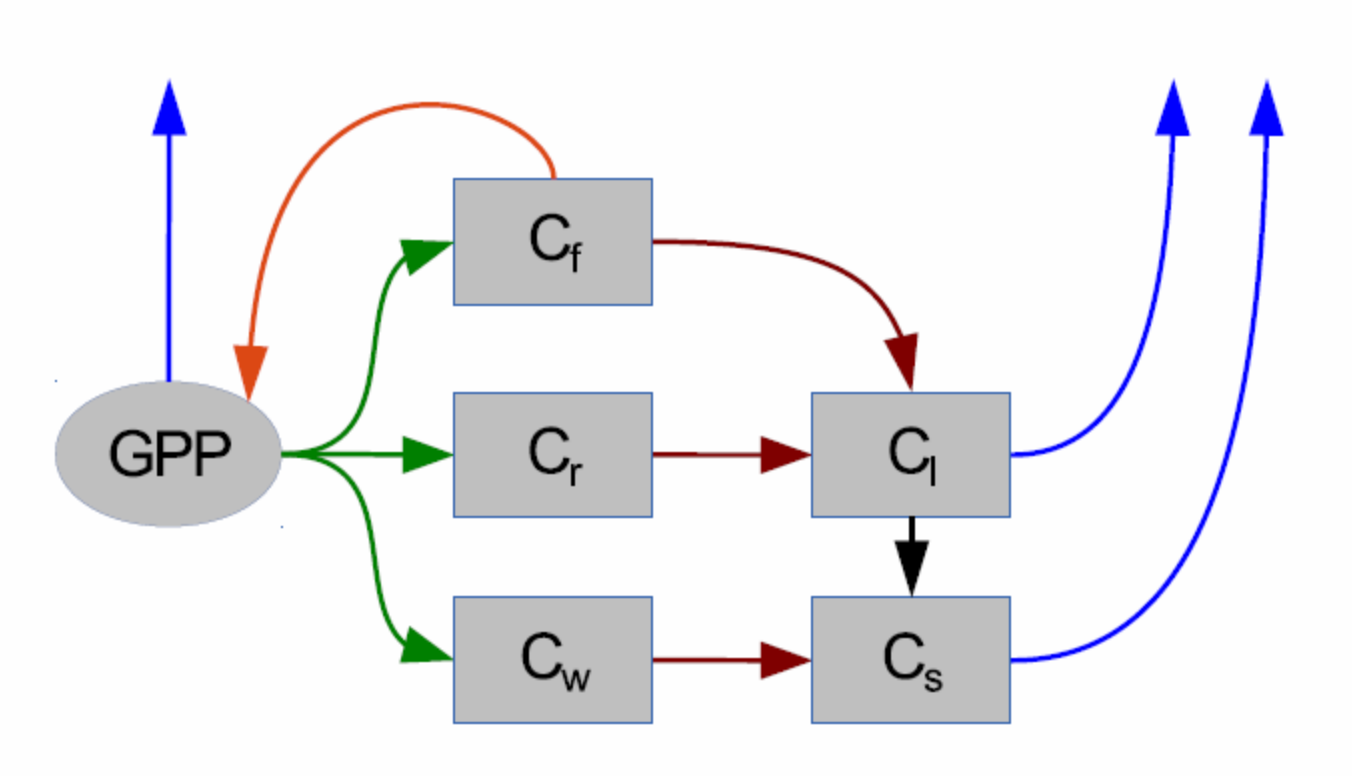
\includegraphics[width=0.5\textwidth]{chapter/chapter5/DALECpic.png}
    \caption{Representation of the carbon fluxes in the DALEC carbon balance model. Green arrows represent C allocation, dark red and black arrows represent litterfall and decomposition fluxes, blue arrows represent respiration fluxes and the light red arrow represents the feedback of foliar carbon to the $GPP$ function. \citep{delahaies2013regularization}}
    \label{fig:DALEC_mod1}
\end{figure}

The model equations for the carbon pools at day $i$ are as follows:
\begin{align}
GPP^{i} &= ACM(C_{fol}^{i-1}, c_{lma}, c_{eff}, \Psi) \label{chap5:d1GPP}
\\C_{fol}^{i}&=C_{fol}^{i-1}+(1-f_{auto})f_{fol}GPP^{i}-\theta_{fol}C_{fol}^{i-1},
\\C_{roo}^{i}&=C_{roo}^{i-1}+(1-f_{auto})(1-f_{fol})f_{roo}GPP^{i}-\theta_{roo}C_{roo}^{i-1}, 
\\C_{woo}^{i}&=C_{woo}^{i-1}+(1-f_{auto})(1-f_{fol})(1-f_{roo})GPP^{i}-\theta_{woo}C_{woo}^{i-1}, 
\\C_{lit}^{i}&=C_{lit}^{i-1}+\theta_{roo}C_{roo}^{i-1}-(\theta_{lit}+\theta_{min})e^{\Theta T^{i-1}}C_{lit}^{i-1}, 
\\C_{som}^{i}&=C_{som}^{i-1}+\theta_{woo}C_{woo}^{i-1}+\theta_{min}e^{\Theta T^{i-1}}C_{lit}^{i-1}-\theta_{som}e^{\Theta T^{i-1}}C_{som}^{i-1}, \label{chap5:d1dalec5}
\end{align}
where $T^{i-1}$ is the daily mean temperature and $\Psi$ represents the meteorological driving data used in the GPP function. Descriptions for each model parameter used in equations \eqref{chap5:d1GPP} to \eqref{chap5:d1dalec5} are shown in table~\ref{chap5:table:D1params}. Further details of this version of DALEC can be found in \cite{williams2005improved}. It is parameterised for data from a young pine stand in Ponderossa, Oregon. The equations used to calculate GPP are included in section~\ref{chap5:sec:ACM}. 

\begin{center}
\scriptsize
\begin{tabular}{| l | l | l | l |}
\hline
Parameter & Description & Value & Range \\ \hline
$\theta_{min}$ & Litter mineralisation rate (day$^{-1}$) & $4.41\times 10^{-6}$ & $10^{-6} - 10^{-2}$ \\ \hline
$f_{auto}$ & Autotrophic respiration fraction & $0.47$ & $0.3 - 0.7$ \\ \hline
$f_{fol}$ & Fraction of GPP allocated to foliage & $0.31$ & $0.01-0.5$ \\ \hline
$f_{roo}$ & Fraction of GPP allocated to fine roots & $0.43$ & $0.01-0.5$ \\ \hline
$\theta_{fol}$ & Foliar carbon turnover rate (day$^{-1}$) & $2.7\times 10^{-3}$ & $10^{-4} - 10^{-1}$ \\ \hline
$\theta_{woo}$ & Woody carbon turnover rate (day$^{-1}$) & $2.06\times 10^{-6}$ & $2.5\times10^{-5} - 10^{-3}$ \\ \hline
$\theta_{roo}$ & Fine root carbon turnover rate (day$^{-1}$) & $2.48\times 10^{-3}$ & $10^{-4} - 10^{-2}$ \\ \hline
$\theta_{lit}$ & Litter carbon turnover rate (day$^{-1}$) & $2.28\times 10^{-2}$ & $10^{-4} - 10^{-1}$ \\ \hline
$\theta_{som}$ & Soil and organic carbon turnover rate (day$^{-1}$) & $2.65\times 10^{-6}$ & $10^{-7} - 10^{-3}$ \\ \hline
$\Theta$ & Temperature dependance exponent factor & $4.147\times 10^{-2}$ & $0.018 - 0.08$ \\ \hline
$C_{fol}$ & Foliar carbon pool ($\text{g C m}^{-2}$) & 58 & $10 - 1000$  \\ \hline
$C_{roo}$ & Fine root carbon pool ($\text{g C m}^{-2}$) & 102 & $10 - 1000$   \\ \hline
$C_{woo}$ & Above and below ground woody carbon pool ($\text{g C m}^{-2}$) & 770 & $100 - 10^{5}$  \\ \hline
$C_{lit}$ & Litter carbon pool ($\text{g C m}^{-2}$) & 40 & $10 - 1000$   \\ \hline
$C_{som}$ & Soil and organic carbon pool ($\text{g C m}^{-2}$) & 9897 & $100 - 2 \times 10^{5}$  \\ 
\hline
\end{tabular}    
\captionof{table}{Parameter and state values for DALEC1, optimised for Metolius forest, Oregon.} \label{chap5:table:D1params}
\end{center}

\subsection{The Aggregated Canopy Model} \label{chap5:sec:ACM}
The aggregated canopy model (ACM) is used in DALEC to calculate GPP. The ACM is a big-leaf, daily time-step model estimating photosynthesis as a function of foliar carbon, leaf mass per area, total daily irradiance, daily temperature values, day length and atmospheric CO\(_{2}\) concentration using the following equations,
\begin{equation}
LAI = \frac{C_f}{c_{lma}} 
\end{equation}
\begin{equation} 
g_c = \frac{|\psi_d|^{a_{10}}}{\frac{1}{2}T_r + a_6~R_{tot}},
\end{equation}
\begin{equation}
p = \frac{c_{eff}~LAI}{g_c}\text{exp}(T_{max}~a_8),
\end{equation}
\begin{equation}
q = a_3 - a_4,
\end{equation}
\begin{equation}
C_i = \frac{1}{2}\bigg[C_a + q - p + \sqrt{(C_a + q + p)^{2} - 4(C_a~q - p~a_3)} \bigg],
\end{equation}
\begin{equation}
E_0 = \frac{a_7~LAI^2}{LAI^2 + a_9},
\end{equation}
\begin{equation}
\delta = -0.408\arccos\bigg(\frac{360~(D+10)}{365}\frac{\pi}{180}\bigg),
\end{equation}
\begin{equation}
s = 24\arccos(-\tan(lat)\tan(\delta))/\pi,
\end{equation}
\begin{equation}
GPP = \frac{E_0~I~g_c~(C_a-C_i)}{E_0~I + g_c~(C_a-C_i)}(a_2~s + a_5),
\end{equation}
where the symbol meanings are shown in table~\ref{chap5:table:acm} with $a_2,\dots ,a_{10}$ being set parameters (values shown in table~\ref{chap5:table:acm_params}). We use the values of the parameters given in \citet{fox2009reflex} as these parameters have been shown to accurately predict GPP for a number of temperate forest sites. The ACM model performs well when tested against other more complex models of photosynthesis \citep{williams1997predicting}. This model can also be driven with estimates of soil-leaf water potential difference and hydraulic resistance; this adds a limit to GPP when the ecosystem is under drought-stress. Alice Holt is a well watered forest so we assume no drought-stress and fix these parameters with values, \(\psi_d = -2.5\) and \(R_{tot} = 1\) \citep{fox2009reflex}.
\begin{center}
\begin{tabular}{| l | l |}
\hline
Symbol & Description \\ \hline
$g_c$ & Canopy conductance $(\text{g C m}^{-2}~\text{day}^{-1})$ \\ \hline
$\psi_d$ & Max soil-leaf water potential difference $(\text{MPa})$ \\ \hline
$T_r$ & Daily temperature range $( ^{o}\text{C})$ \\ \hline
$R_{tot}$ & Total plant-soil hydraulic resistance $(\text{MPa}~\text{m}^2~\text{s}~\text{mmol}^{-1})$ \\ \hline
$c_{lma}$ & Leaf mass per area $(\text{g C m}^{-2})$  \\ \hline
$LAI$ & Leaf area index $(\text{m}^2~\text{m}^{-2})$ \\ \hline
$c_{eff}$ &canopy use efficiency parameter $(\text{g C m}^{-2})$  \\ \hline
$T_{max}$ & Maximum daily temperature $( ^{o}\text{C})$  \\ \hline
$C_a$ & Atmospheric CO$_2$ concentration $(\mu~\text{mol mol}^{-1})$ \\ \hline
$C_i$ & CO$_2$ concentration at site of carboxylation $(\mu~\text{mol mol}^{-1})$ \\ \hline
$E_0$ & Canopy level quantum yield $(\text{g C MJ}^{-1}~\text{m}^{-2}~\text{day}^{-1})$ \\ \hline
$\delta$ & Solar declination $(\text{radians})$ \\ \hline
$D$ & Day of year \\ \hline
$s$ & Day length $(\text{hrs})$ \\  \hline  
$lat$ & Site latitude $( ^{o})$ \\ \hline
$I$ & Irradiance $(\text{MJ m}^{-2}~\text{day}^{-1})$ \\ 
\hline
\end{tabular}    
\captionof{table}{Symbols used in ACM.} \label{chap5:table:acm}
\end{center}

\begin{center}
\begin{tabular}{| l | l |}
\hline
Parameter & Value \\ \hline
$a_2$ & 0.0155 \\ \hline
$a_3$ & 1.526 \\ \hline
$a_4$ & 324.1 \\ \hline
$a_5$ & 0.2017 \\ \hline
$a_6$ & 1.315 \\ \hline
$a_7$ & 2.595 \\ \hline
$a_8$ & 0.037 \\ \hline
$a_9$ & 0.2268 \\ \hline
$a_{10}$ & 0.9576 \\
\hline
\end{tabular}    
\captionof{table}{Parameter values in ACM.} \label{chap5:table:acm_params}
\end{center}

\subsection{The DALEC2 model} \label{chap5:sec:dalec2}

The DALEC2 model is a new, slightly more complex version of the DALEC1 model describing the carbon balance of a forest ecosystem \citep{Bloom2015}. The model is constructed of six carbon pools (labile ($C_{lab}$), foliage ($C_f$), fine roots ($C_r$), woody stems and coarse roots ($C_w$), fresh leaf and fine root litter ($C_l$) and soil organic matter and coarse woody debris ($C_s$)) linked via fluxes. The aggregated canopy model (ACM) \citep{williams1997predicting} is again used to calculate daily gross primary production ($GPP$) of the forest, taking meteorological driving data and the modelled leaf area index (a function of $C_f$) as arguments. Figure~\ref{fig:DALEC_mod} shows a schematic of how the carbon pools are linked in DALEC2.   

\begin{figure}[ht]
    \centering
    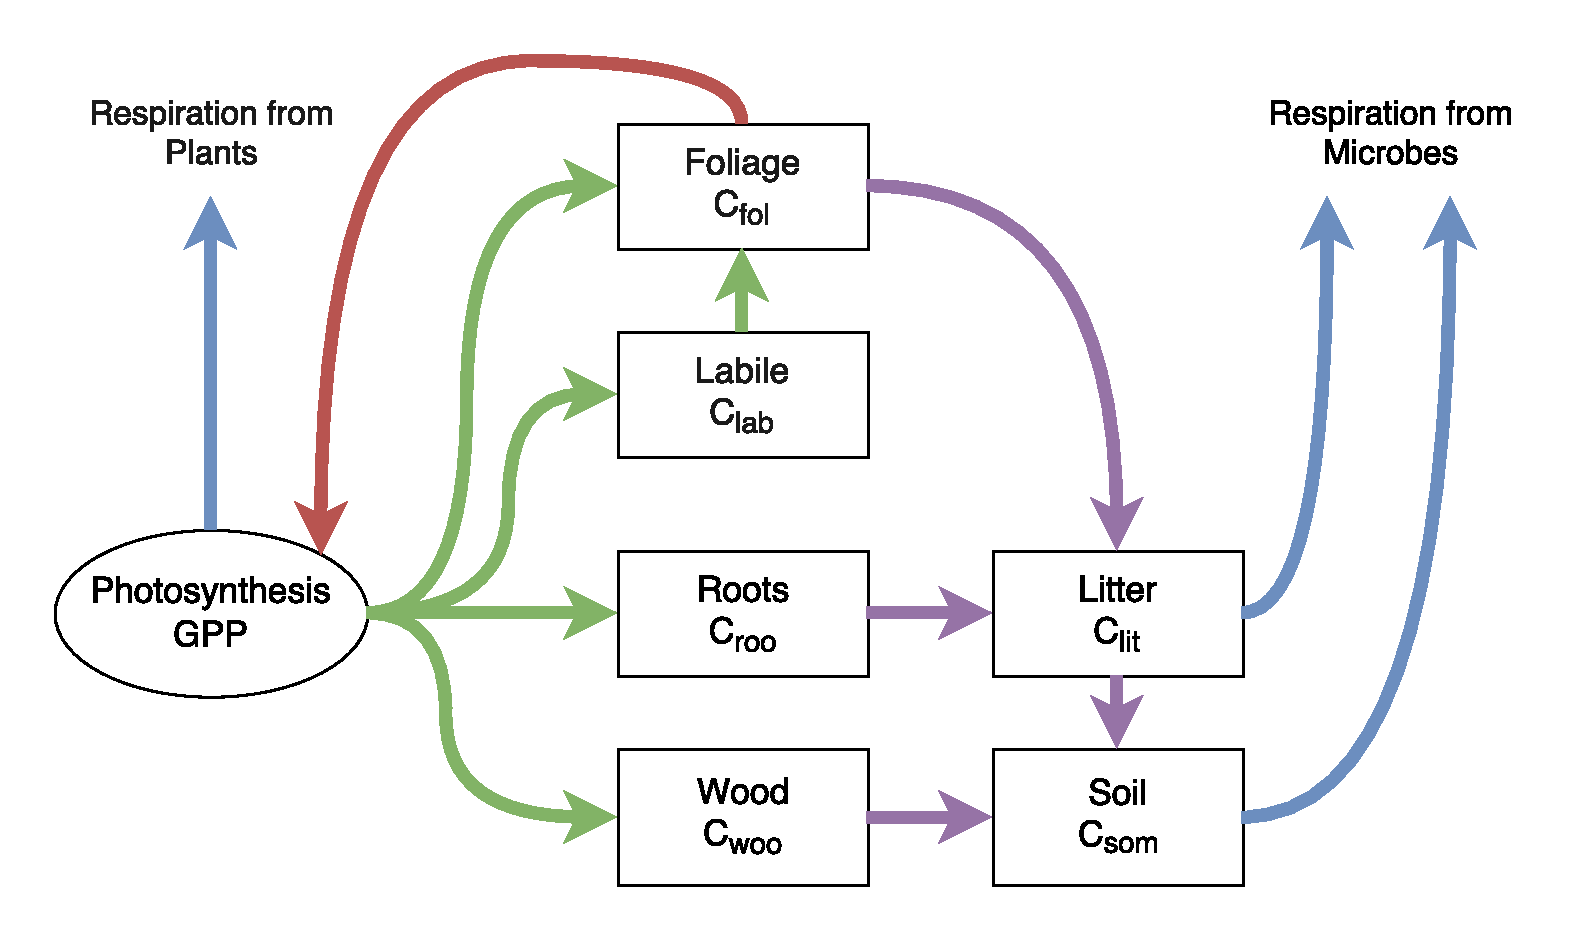
\includegraphics[width=0.5\textwidth]{chapter/chapter5/dalec2diag.pdf}
    \caption{Representation of the fluxes in the DALEC2 carbon balance model. Green arrows represent C allocation, purple arrows represent litter fall and decomposition fluxes, blue arrows represent respiration fluxes and the red arrow represents the influence of leaf area index in the GPP function.} \label{fig:DALEC_mod}
\end{figure}

The model equations for the carbon pools at day $i$ are as follows:

\begin{align}
GPP^{i} &= ACM(C_{fol}^{i-1}, c_{lma}, c_{eff}, \Psi) \label{chap5:d2GPP}
\\C_{lab}^{i}&=C_{lab}^{i-1}+(1-f_{auto})(1-f_{fol})f_{lab}GPP^{i}-\Phi _{on}C_{lab}^{i-1}, \label{daleclab}
\\C_{fol}^{i}&=C_{fol}^{i-1}+\Phi_{on}C_{lab}^{i-1}+(1-f_{auto})f_{fol}GPP^{i}-\Phi_{off}C_{fol}^{i-1}, \label{dalec1}
\\C_{roo}^{i}&=C_{roo}^{i-1}+(1-f_{auto})(1-f_{fol})(1-f_{lab})f_{roo}GPP^{i}-\theta_{roo}C_{roo}^{i-1}, 
\\C_{woo}^{i}&=C_{woo}^{i-1}+(1-f_{auto})(1-f_{fol})(1-f_{lab})(1-f_{roo})GPP^{i}-\theta_{woo}C_{woo}^{i-1}, 
\\C_{lit}^{i}&=C_{lit}^{i-1}+\theta_{roo}C_{roo}^{i-1}+\Phi_{off}C_{fol}^{i-1}-(\theta_{lit}+\theta_{min})e^{\Theta T^{i-1}}C_{lit}^{i-1}, 
\\C_{som}^{i}&=C_{som}^{i-1}+\theta_{woo}C_{woo}^{i-1}+\theta_{min}e^{\Theta T^{i-1}}C_{lit}^{i-1}-\theta_{som}e^{\Theta T^{i-1}}C_{som}^{i-1}, \label{chap5:d2dalec5}
\end{align}
where $T^{i-1}$ is the daily mean temperature, $\Psi$ represents the meteorological driving data used in the $GPP$ function and $\Phi_{on} / \Phi_{off}$ are functions controlling leaf-on and leaf-off. Descriptions for each model parameter used in equations \eqref{chap5:d2GPP} to \eqref{chap5:d2dalec5} are included in table~\ref{chap5:table:xbvars}. DALEC2 differs from the original DALEC in that it can be parameterised for both deciduous and evergreen sites with $\Phi_{on}$ and $\Phi_{off}$ being able to reproduce the phenology of either type of site. From table~\ref{chap5:table:D1params} and ~\ref{chap5:table:xbvars} we can see that whereas DALEC1 has 10 parameters and 5 state variables, DALEC2 has 17 parameters and 6 state variables. Further details of this version of DALEC can be found in \cite{Bloom2015}. 

\begin{table}[ht] 
\begin{center}
\scriptsize
	\begin{tabular}{| l | p{4.5cm} | l | l |}
	\hline
	Parameter & Description & Prior estimate ($\textbf{x}^{b}$)  & Range \\ \hline
$\theta_{min}$ & Litter mineralisation rate (day$^{-1}$) & $9.810\times 10^{-4}$ & $10^{-5} - 10^{-2}$ \\ \hline
$f_{auto}$ & Autotrophic respiration fraction & $5.190\times 10^{-1}$ &  $0.3 - 0.7$  \\ \hline
$f_{fol}$ & Fraction of GPP allocated to foliage & $1.086\times 10^{-1}$ & $0.01-0.5$ \\ \hline
$f_{roo}$ & Fraction of GPP allocated to fine roots & $4.844\times 10^{-1}$ & $0.01-0.5$ \\ \hline
$c_{lspan}$ & Determines annual leaf loss fraction & $1.200\times 10^{0} $ & $1.0001 - 10$ \\ \hline
$\theta_{woo}$ & Woody carbon turnover rate (day$^{-1}$) & $1.365\times 10^{-4}$ & $2.5\times10^{-5} - 10^{-3}$ \\ \hline
$\theta_{roo}$ & Fine root carbon turnover rate (day$^{-1}$) & $3.225\times 10^{-3}$ & $10^{-4} - 10^{-2}$ \\ \hline
$\theta_{lit}$ & Litter carbon turnover rate (day$^{-1}$) & $3.442\times 10^{-3}$ & $10^{-4} - 10^{-2}$ \\ \hline
$\theta_{som}$ & Soil and organic carbon turnover rate (day$^{-1}$) & $1.113\times 10^{-4}$ & $10^{-7} - 10^{-3}$ \\ \hline
$\Theta$ & Temperature dependance exponent factor & $4.147\times 10^{-2}$ & $0.018 - 0.08$ \\ \hline
$c_{eff}$ & Canopy efficiency parameter & $7.144\times 10^{1}$ & $10 - 100$ \\ \hline
$d_{onset}$ & Leaf onset day (day) & $1.158\times 10^{2}$ & $1 - 365$ \\ \hline
$f_{lab}$ & Fraction of GPP allocated to labile carbon pool & $3.204\times 10^{-1}$ & $0.01 - 0.5$ \\ \hline
$c_{ronset}$ & Labile carbon release period (days) & $4.134\times 10^{1}$ & $10 - 100$ \\ \hline
$d_{fall}$ & Leaf fall day (day) & $2.205\times 10^{2}$ & $1 - 365$ \\ \hline
$c_{rfall}$ & Leaf-fall period (days) & $1.168\times 10^{2}$ & $10 - 100$ \\ \hline
$c_{lma}$ & Leaf mass per area ($\text{g C m}^{-2}$) & $1.285\times 10^{2}$ & $10 - 400$ \\ \hline
$C_{lab}$ & Labile carbon pool ($\text{g C m}^{-2}$) & $1.365\times 10^{2}$ & $10 - 1000$ \\ \hline
$C_{fol}$ & Foliar carbon pool ($\text{g C m}^{-2}$) & $6.864\times 10^{1}$ & $10 - 1000$ \\ \hline
$C_{roo}$ & Fine root carbon pool ($\text{g C m}^{-2}$) & $2.838\times 10^{2}$ & $10 - 1000$ \\ \hline
$C_{woo}$ & Above and below ground woody carbon pool ($\text{g C m}^{-2}$) & $6.506\times 10^{3}$ & $100 - 10^{5}$ \\ \hline
$C_{lit}$ & Litter carbon pool ($\text{g C m}^{-2}$) & $5.988\times 10^{2}$ & $10 - 1000$ \\ \hline
$C_{som}$ & Soil and organic carbon pool ($\text{g C m}^{-2}$) & $1.936\times 10^{3}$ & $100 - 2 \times 10^{5}$  \\ \hline
	\end{tabular}
	\caption{Parameter and state values for DALEC2.}
	\label{chap5:table:xbvars}
\end{center} 
\end{table}


\section{Data}

As part of this PhD an extended period of time has been spent at the Alice Holt Research Station (Hampshire, UK) working with Forest Research (the research arm of the UK Forestry Commission). After initially completing one year of an ongoing field campaign to measure stem respiration using an infra-red gas analyser, a measurement campaign was designed to produce a set of observations for use in this PhD project. This involved the establishment and sampling of three transects throughout the Straits Inclosure (part of the Alice Holt forest). The establishment of these transects and measurements are outlined in section~\ref{chap4:sec:transect} to \ref{chap4:sec:pcq}.

\subsection{Alice Holt research site} \label{chap4:sec:aliceholt}

The Alice Holt Forest is a research forest area managed by the UK Forestry Commission located in Hampshire, SE England. Forest Research have been operating a $\text{CO}_{2}$ flux measurement tower in a portion of the forest, the Straits Inclosure, continuously since 1998. The Straits Inclosure is a $90~\text{ha}$ area of deciduous broadleaved plantation woodland located on a surface water gley soil and was initially planted with oak in the 1820s \citep{schlich1905working} and then replanted in the 1930s. The majority of the canopy trees are oak (\textit{Quercus robur} L.), with an understory of hazel (\textit{Corylus avellana} L.) and hawthorn (\textit{Crataegus monogyna} Jacq.) \citep{pitman2001leaf}, but there is a small area of conifers (\textit{Pinus nigra} ssp. \textit{laricio} (Maire) and \textit{P. sylvestris} L.) within the tower measurement footprint area depending on wind direction. An aerial photograph of the site is shown in Figure~\ref{chap4:fig:ah_aerial_photo}. The Straits Inclosure is a flat area at an altitude of approximately 80m, surrounded by mixed lowland woods and both arable and pasture agricultural land. In \citet{wilkinson2012inter} an analysis of stand-scale $30$ minute average net $\text{CO}_{2}$ fluxes (NEE) from 1998-2011 for the Straits Inclosure found a mean annual NEE of \(-486~\text{g C m}^{-2}~\text{yr}^{-1}\) and demonstrated the forest was a substantial sink of carbon. This study also includes further details about the research site. 

As part of the management regime, the Straits Inclosure is subject to thinning, whereby a proportion of trees are removed from the canopy in order to reduce competition and improve the quality of the final tree crop. An intermediate thinning method is used with a portion of both subdominant and dominant trees being removed from the stand \citep{kerr2011thinning}. The whole of the stand was thinned in 1995. Subsequently the eastern side of the Straits was thinned in 2007 and then the western side in 2014. The flux tower at the site is situated on the boundary between these two sides. This allows for the use of a footprint model to split the flux record and thus analyse the effect of this disturbance on carbon fluxes at the site. In \citet{wilkinson2015effects} a statistical analysis of the eddy covariance flux record found that there was no significant effect on the net carbon uptake of the eastern side after thinning in 2007. In Chapter~\ref{chap:disturbance} we focus on the effect of disturbance on the western side after thinning in 2014. We therefore refer to the western side as ``thinned'' forest and the eastern side as ``unthinned'' forest.   


\begin{figure}[ht]
    \centering
    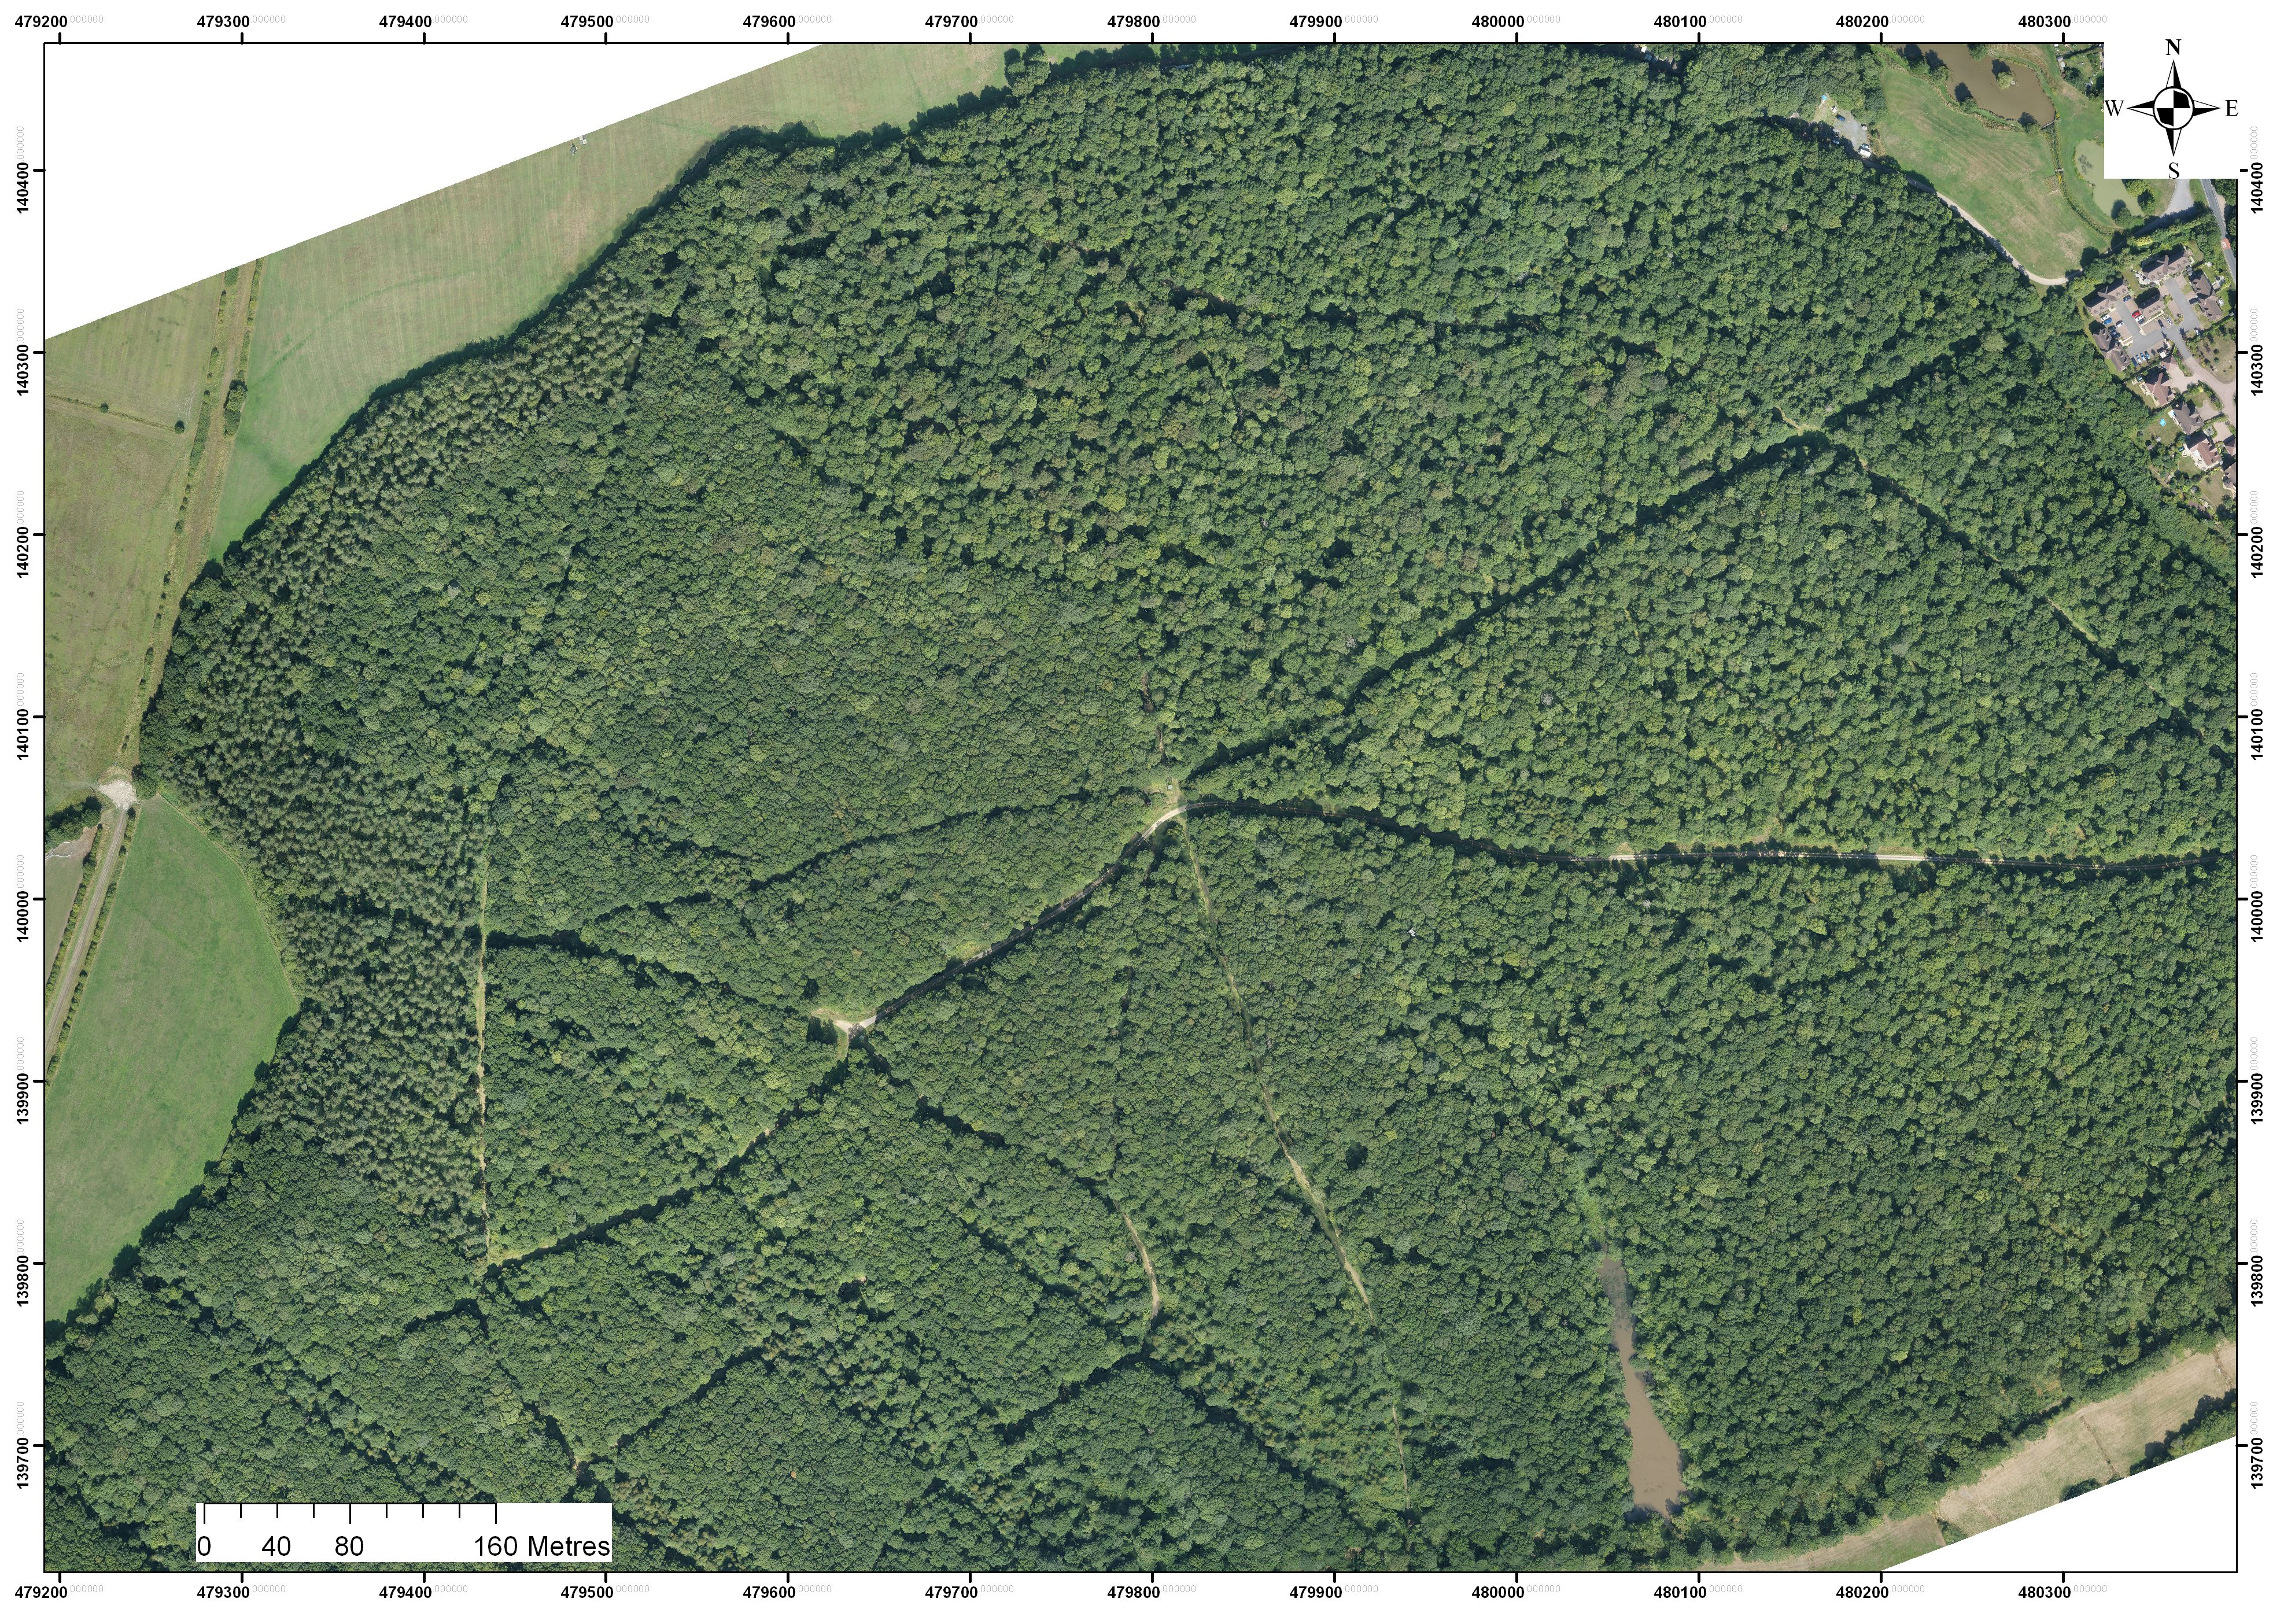
\includegraphics[width=0.8\textwidth]{chapter/chapter4/AP1_2013.jpg}
    \caption{The Straits Inclosure research site in 2013. Source: Forest Research} \label{chap4:fig:ah_aerial_photo}
\end{figure}

\subsection{Establishment of sampling points} \label{chap4:sec:transect}

For this fieldwork transects were designed to join up existing mensuration plots where measurements of woody biomass are made by Forest Research. This allowed for comparison with historic observations. Sampling points were set at 10m intervals along the transect, giving 435 points in total. These are shown in Figure~\ref{chap4:fig:transects}. The GeoPy Python package was used to calculated the exact latitude and longitude of each sampling point for the 3 transects. These locations were then entered into a GPS unit. When establishing the transects, fluorescent spray paint was used to mark trees closest to each sampling point as shown on the GPS (see Figure~\ref{chap4:fig:pink_tree}). As parts of the forest site were extremely dense with vegetation, a pair of loppers were used to clear a path in some areas to allow for the establishment of relatively straight transects. Having all transect points numbered (with corresponding latitude and longitude value) allowed for comparison between methods and the splitting of observations between distinct sections of the forest site. 


\begin{figure}[ht]
    \centering
    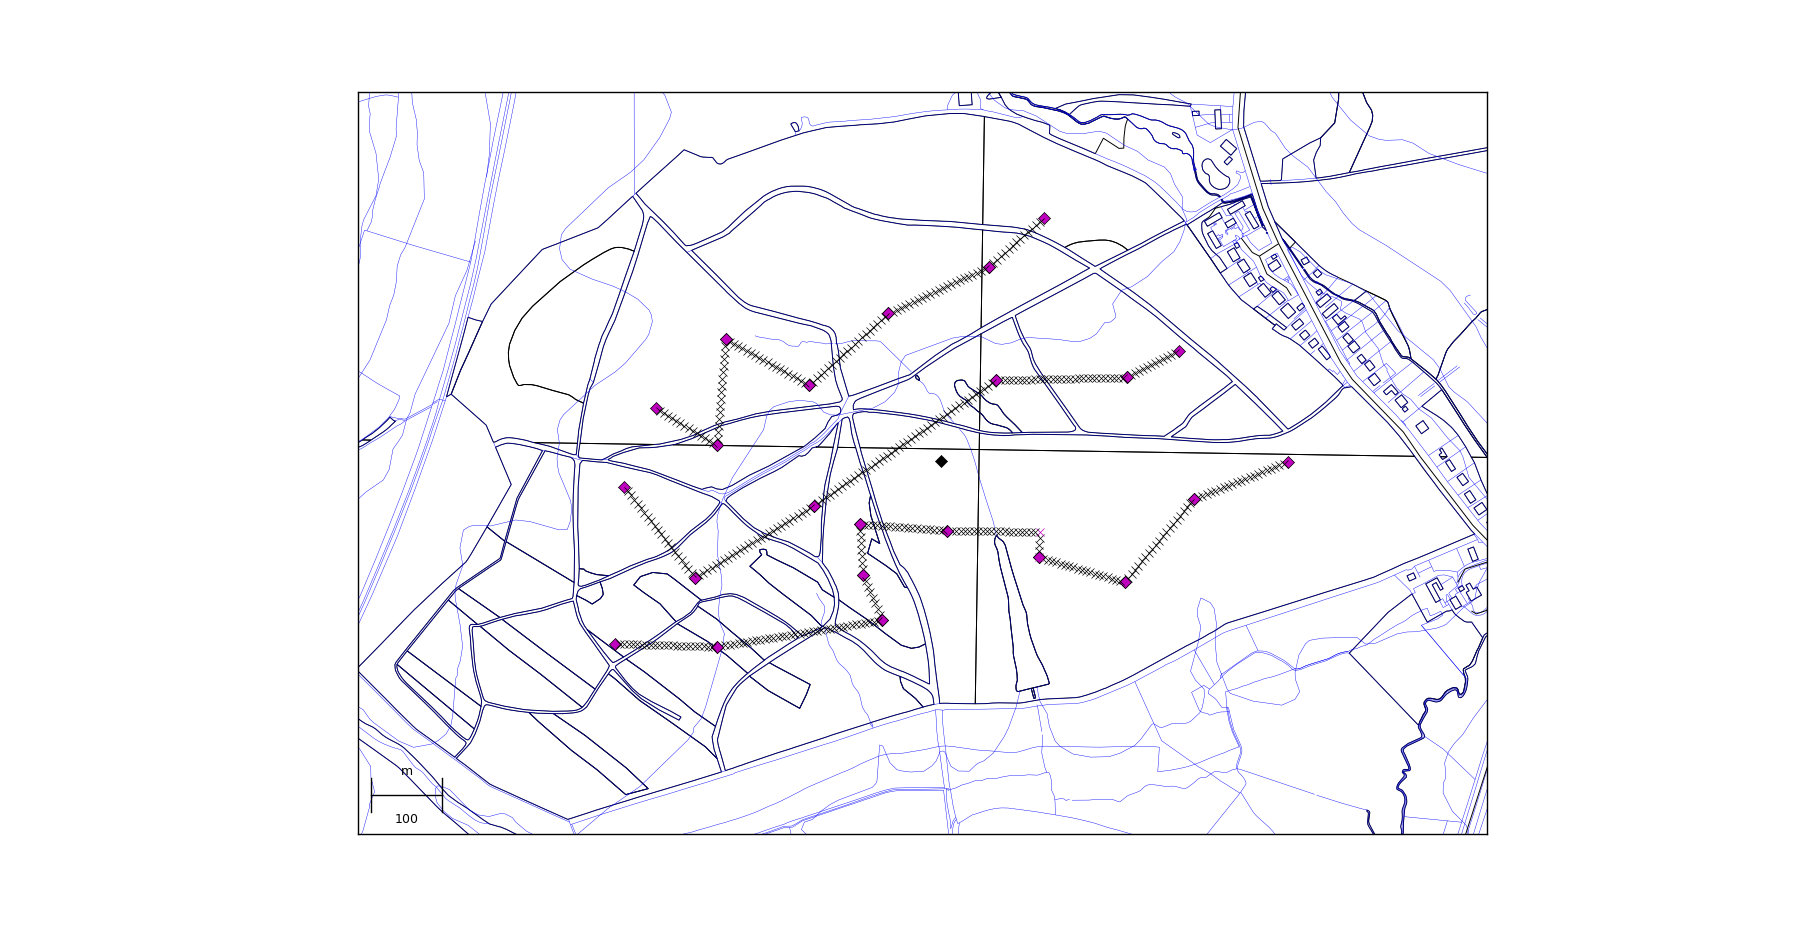
\includegraphics[width=\textwidth]{chapter/chapter4/straitsmap_threet_10m.png}
    \caption{Sampling transects. Black crosses: sampling points at 10m intervals, pink diamonds: Forest Research mensuration plots, black diamond: Forest Research flux tower.} \label{chap4:fig:transects}
\end{figure}

\begin{figure}[ht]
    \centering
    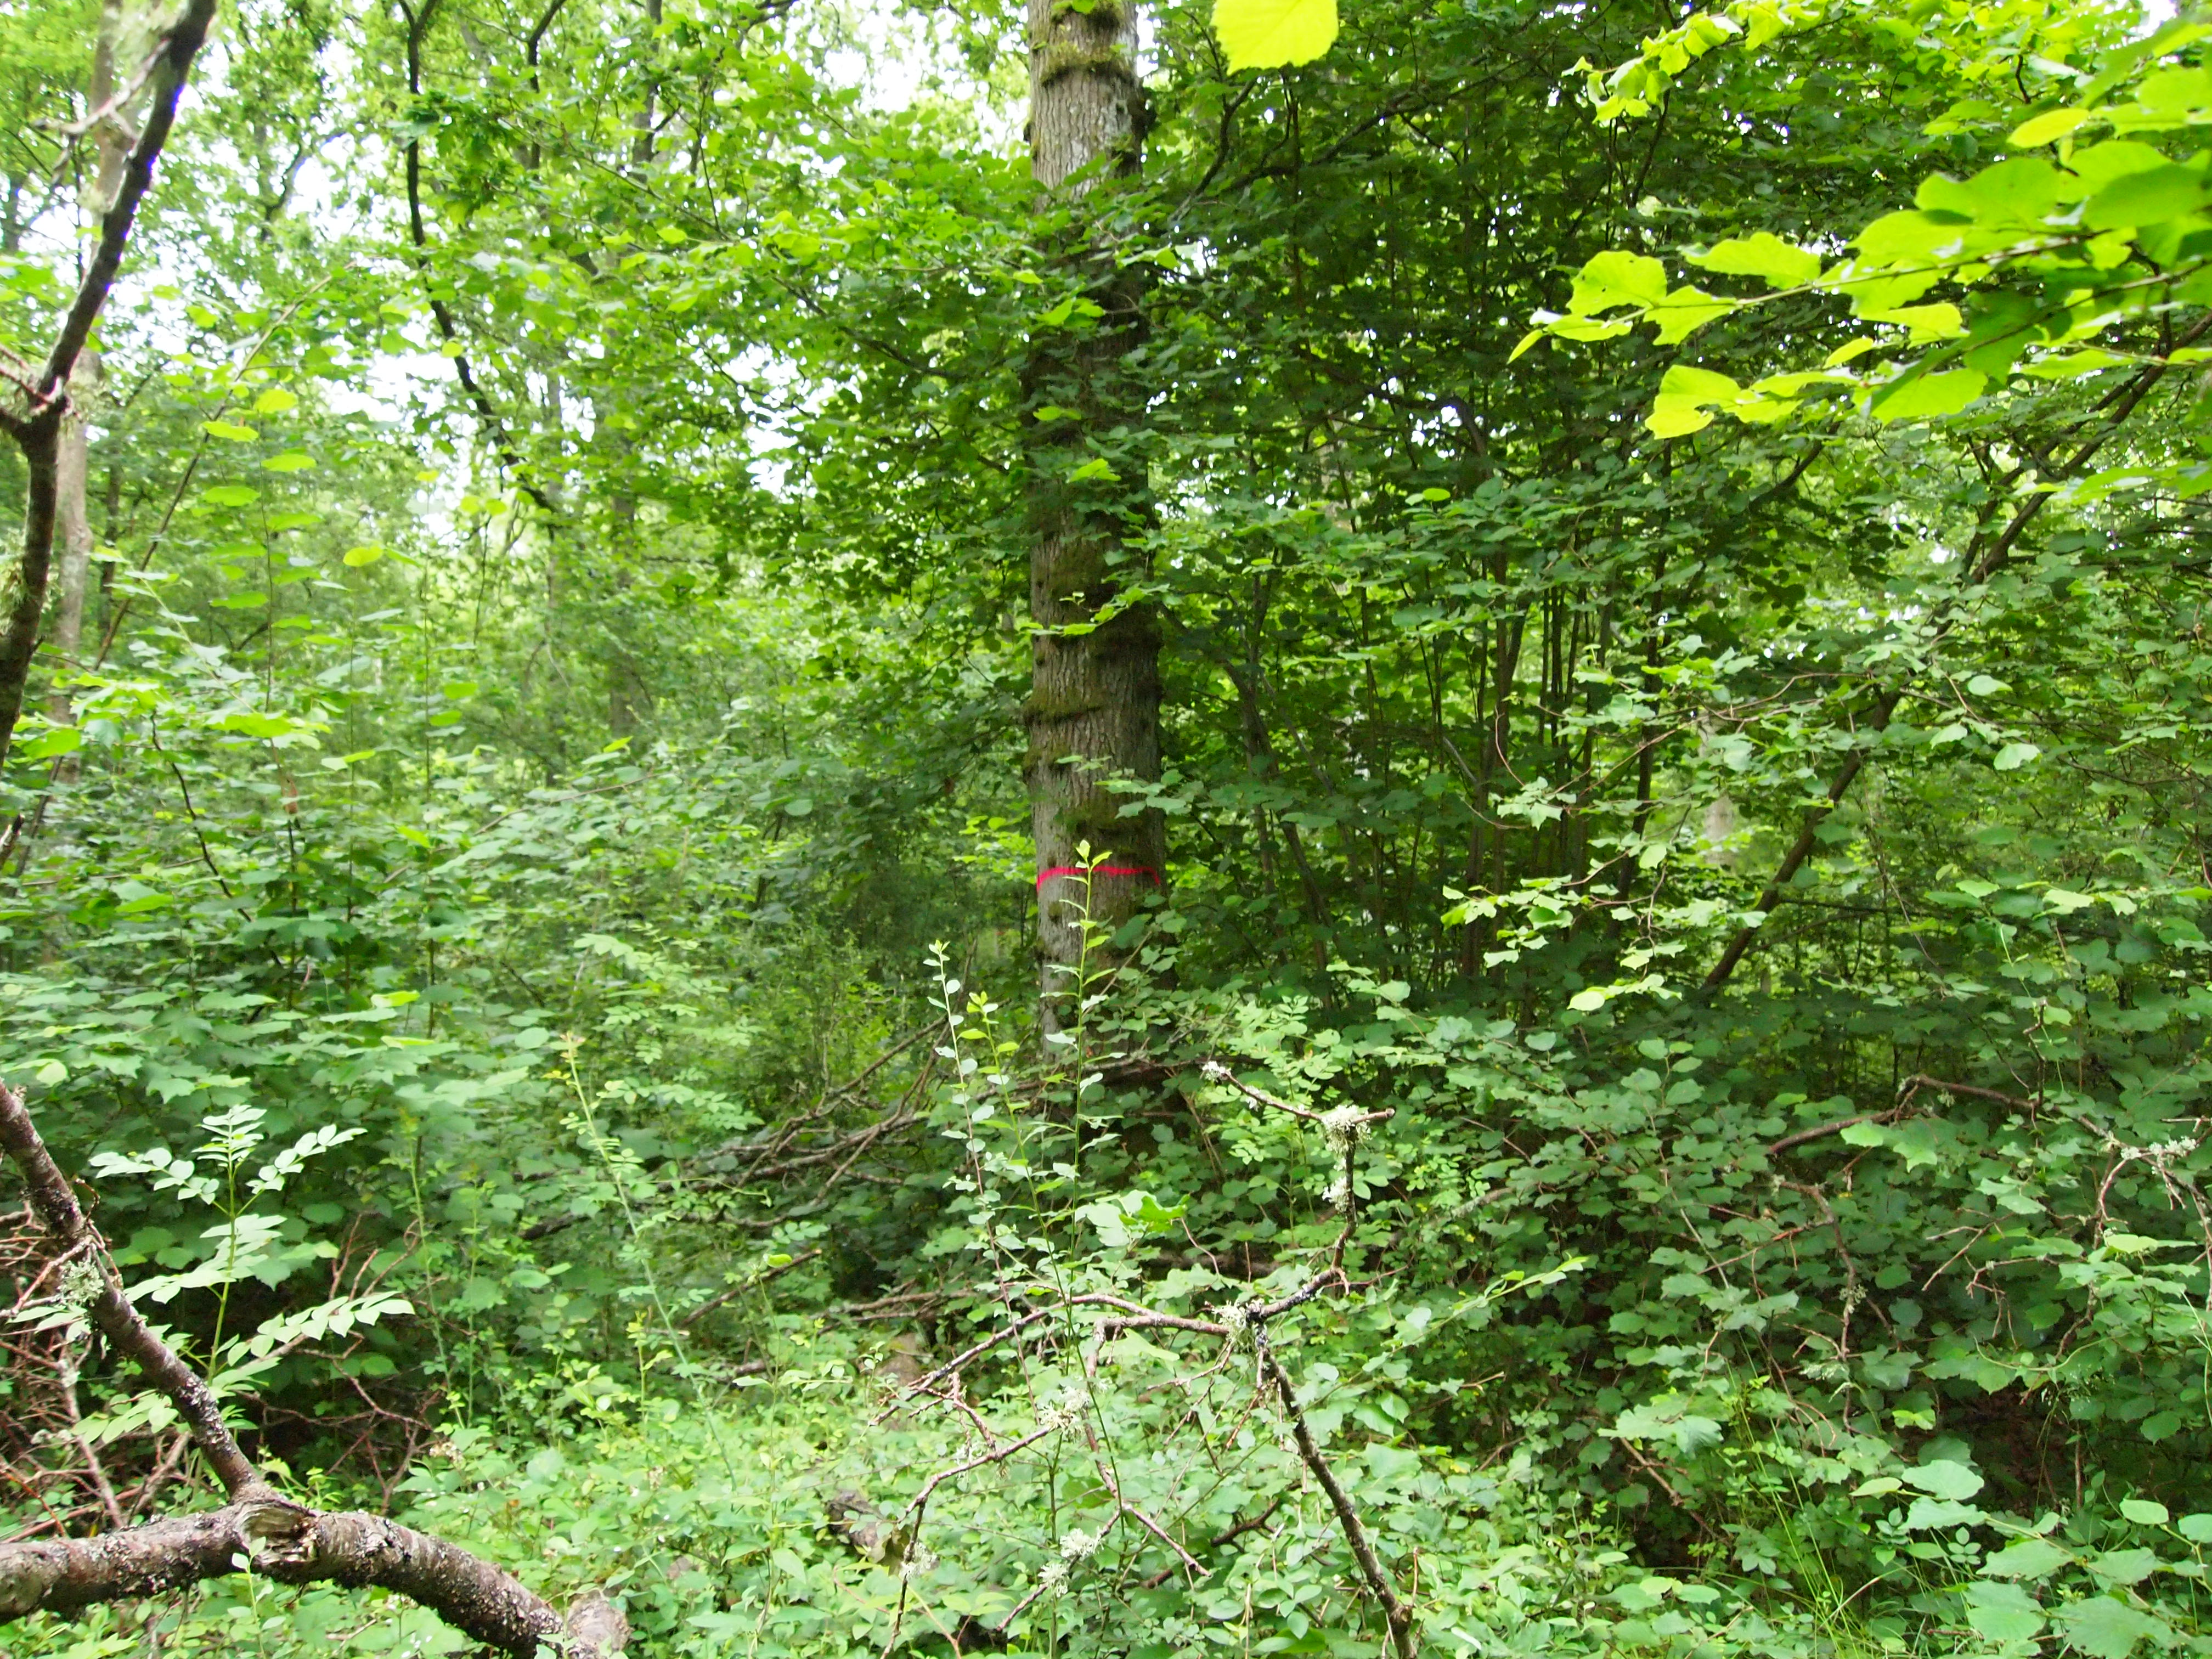
\includegraphics[width=0.8\textwidth]{chapter/chapter4/291E.jpg}
    \caption{Sampling point 291, showing fluorescent spray paint used to mark sampling points.} \label{chap4:fig:pink_tree}
\end{figure}

\subsection{Leaf area index observations}

Leaf Area Index (LAI) is an important variable in relation to the amount of CO\(_2\) an ecosystem can remove from the atmosphere through photosynthesis. LAI is defined as the area of leaves per unit area of ground. Three different methods were used to estimate peak LAI (July - September) for the year 2015 along the three transects at different sampling intervals.

\subsubsection{Ceptometer}

A Decagon LP-80 ceptometer and an additional Photosynthetically Active Radiation (PAR) sensor were used to measure LAI. Here we measure below canopy PAR using the ceptometer while logging above canopy PAR using a PAR sensor and data logger positioned outside the canopy. We can then calculate LAI using the above and below canopy readings. The ceptometer represents the quickest method for estimating LAI, we therefore took readings with the ceptometer at every sampling point over two walks of the transects, giving us 870 observations in total.

In order to be sure that the PAR readings from the ceptometer and external PAR sensor were consistent, we calibrated the PAR sensor against the ceptometer. This was done by leaving both the PAR sensor and ceptometer out logging next to each other every 10 seconds for a day in the Alice Holt Research Station meteorological sampling square. We can then calibrate the output of the PAR sensor with that of the ceptometer, as shown in Figure~\ref{chap4:fig:par_calib}. 

\begin{figure}[ht]
    \centering
    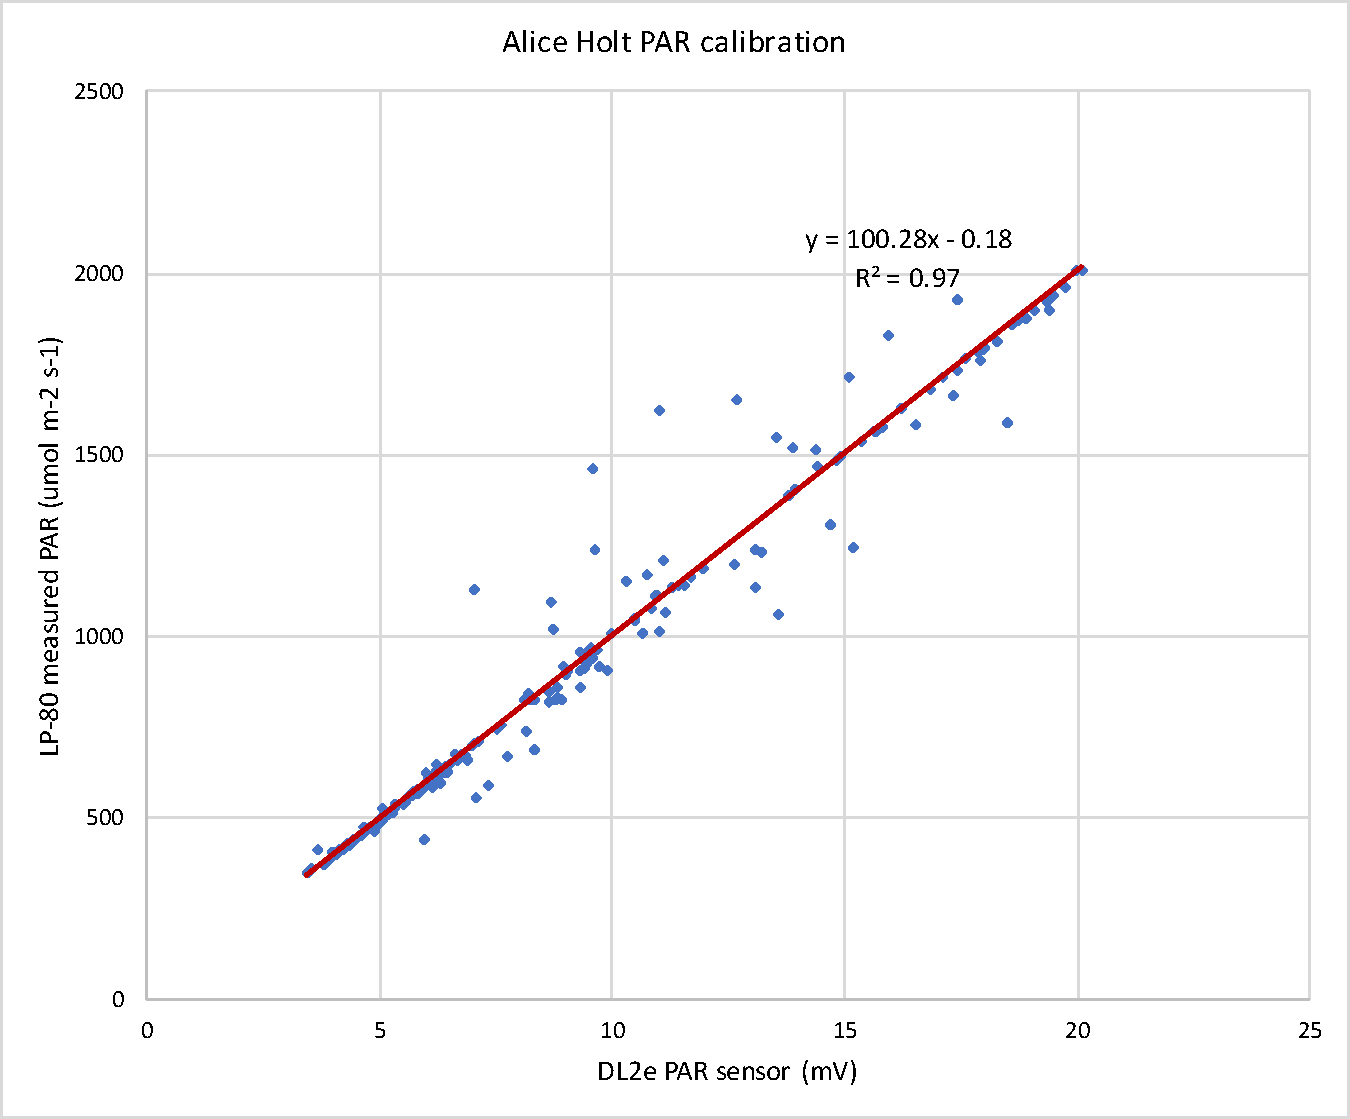
\includegraphics[width=0.8\textwidth]{chapter/chapter4/AH_PAR.pdf}
    \caption{Calibration of above canopy Photosynthetically Active Radiation (PAR) sensor (measuring in mV) with LP-80 ceptometer measured PAR (\(\mu \text{mol}~\text{m}^{-2}~\text{s}^{-1} \)).} \label{chap4:fig:par_calib}
\end{figure}

Once the PAR sensor was calibrated, measurements could be made along the transects. The PAR sensor positioned outside of the canopy was logged every 5 seconds using a Delta-T DL2e data logger, at the start of every set of measurements the clock on the data logger and ceptometer were synchronised to ensure comparison of measurements made at the same time. After sampling the transects we had a set of above canopy and below canopy PAR readings corresponding to each sampling point for both walks of the transects. We use the same calculation for LAI as given in the Decagon LP-80 manual. This is using a simple model of radiation transmission and scattering successfully tested against the more complex model of \citet{norman1975photosynthesis}. The equation used to calculate LAI is,
\begin{equation}
LAI = \frac{((1-\frac{1}{2K})f_b - 1)\text{ln}\tau}{A(1-0.47f_b)},
\end{equation} 
where \(K\) is the extinction coefficient, \(f_b\) is the beam fraction, \(\tau = \frac{\text{below canopy PAR}}{\text{above canopy PAR}}\) and \(A = 0.283 + 0.785a - 0.159 a^2\) (where $a$ is the leaf absorptivity, assumed to be 0.9 by Decagon). We assume a simple extinction coefficient of \(K=\frac{1}{2\text{cos}\theta}\), where \(\theta\) is the solar zenith angle. We took the mean of the two LAI observations at each point to give as an estimate to the peak LAI for the year 2015. We can see the LAI estimate for the Straits Inclosure in Figure~\ref{chap4:fig:cept_lai}. 

\begin{figure}[ht]
    \centering
    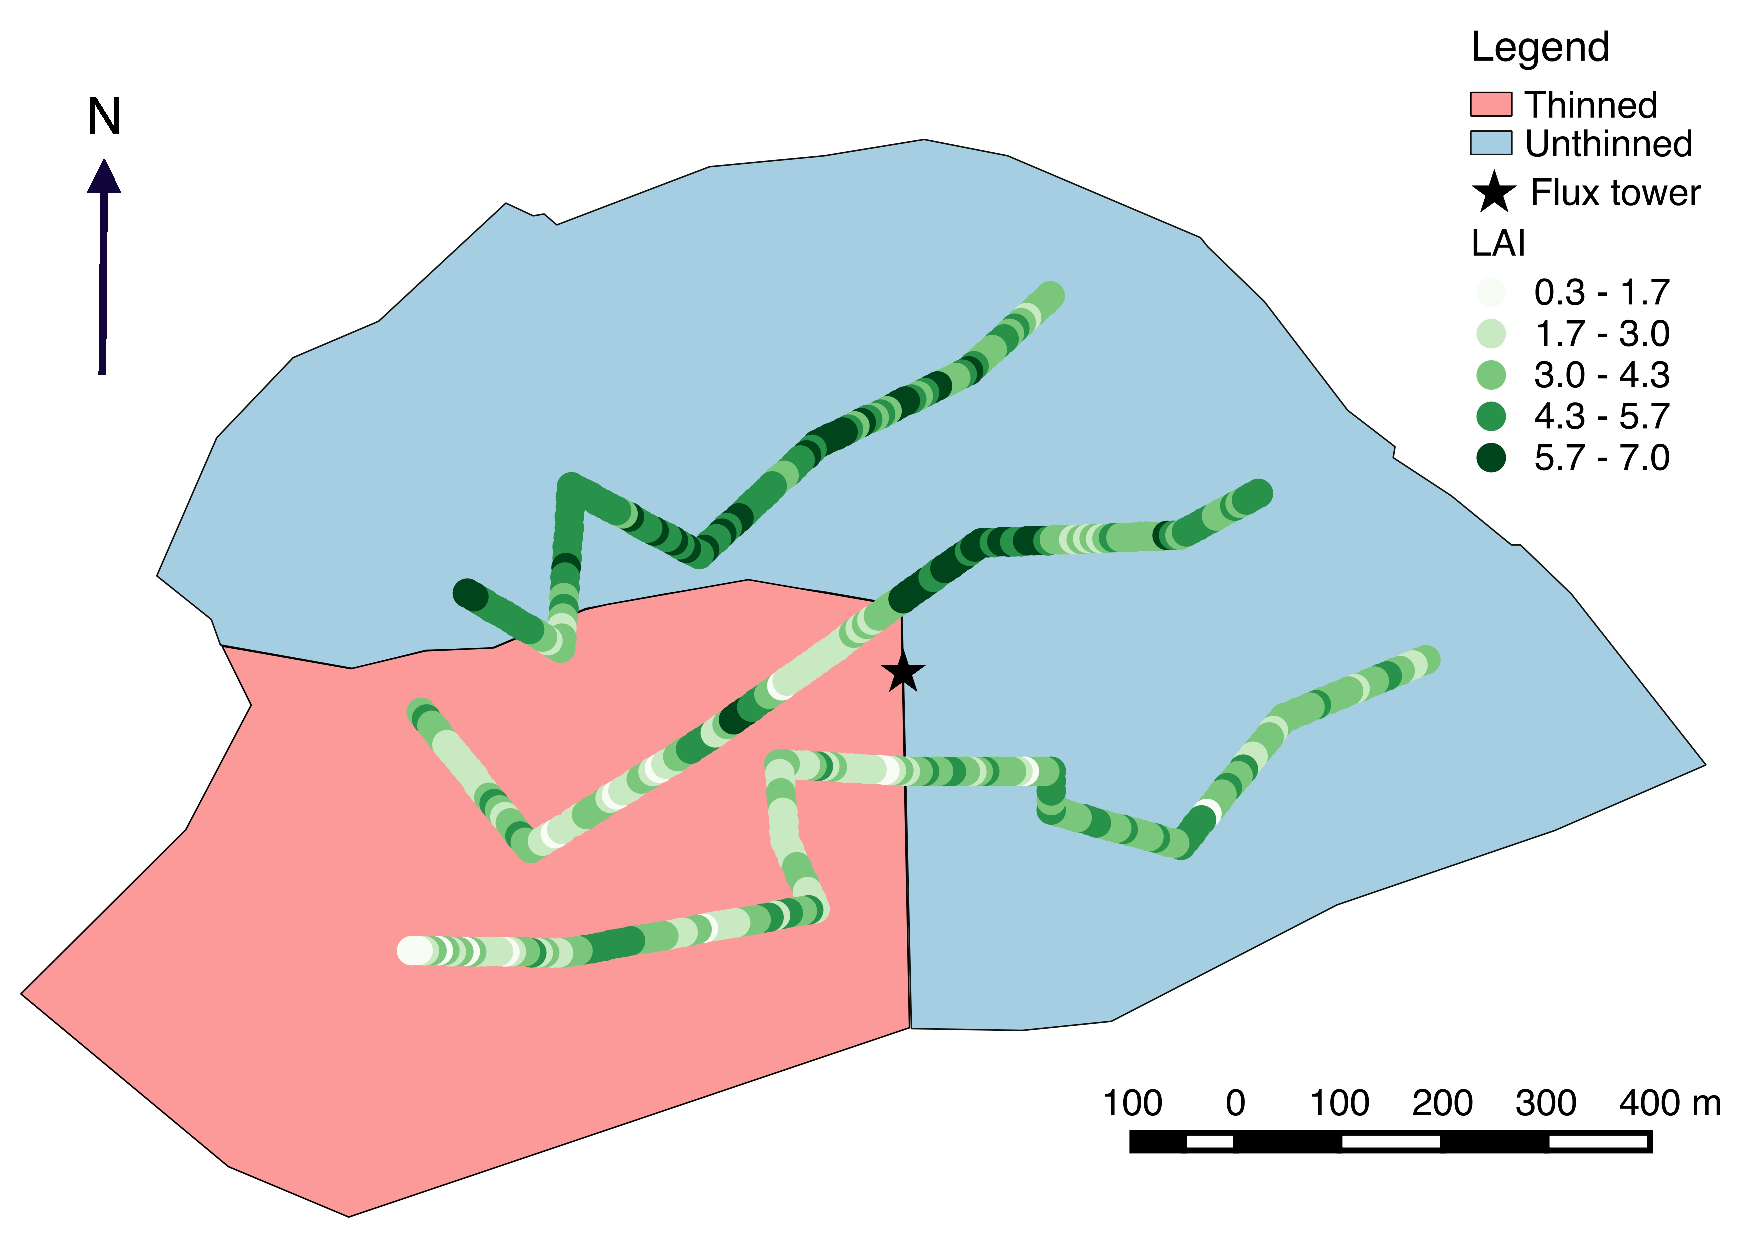
\includegraphics[width=0.8\textwidth]{chapter/chapter4/lai_cept.pdf}
    \caption{Ceptometer derived LAI for 2015, Alice Holt.} \label{chap4:fig:cept_lai}
\end{figure}

\subsubsection{Hemispherical photographs} \label{chap4:sec:hemi_photos}

The second method used to measure LAI was hemispherical photography. Hemispherical photographs show a complete view of the sky in all directions. From these images we use the HemiView software \citep{rich1999hemiview} which calculates the proportion of visible sky as a function of sky direction (gap fraction) which it then uses to calculate LAI \citep{Jonckheere2004}. Hemispherical photographs were taken every 50m along the transects, giving a total of 89 images. It is important to ensure that hemispherical photographs are taken in overcast conditions so that the sun does not mask areas of leaf area. It is important to note that we did not remove tree trunks and branches from our calculation of LAI with HemiView so that we are actually calculating plant area index. The impacts of this assumption are discussed in section~\ref{chap4:sec:lai_comp}. In Figure~\ref{chap4:fig:hemiphotos} we show an example of two hemispherical photographs taken in different areas of the Straits Inclosure.

\begin{figure}[ht]
\centering
\begin{subfigure}{.5\textwidth}
  \centering
  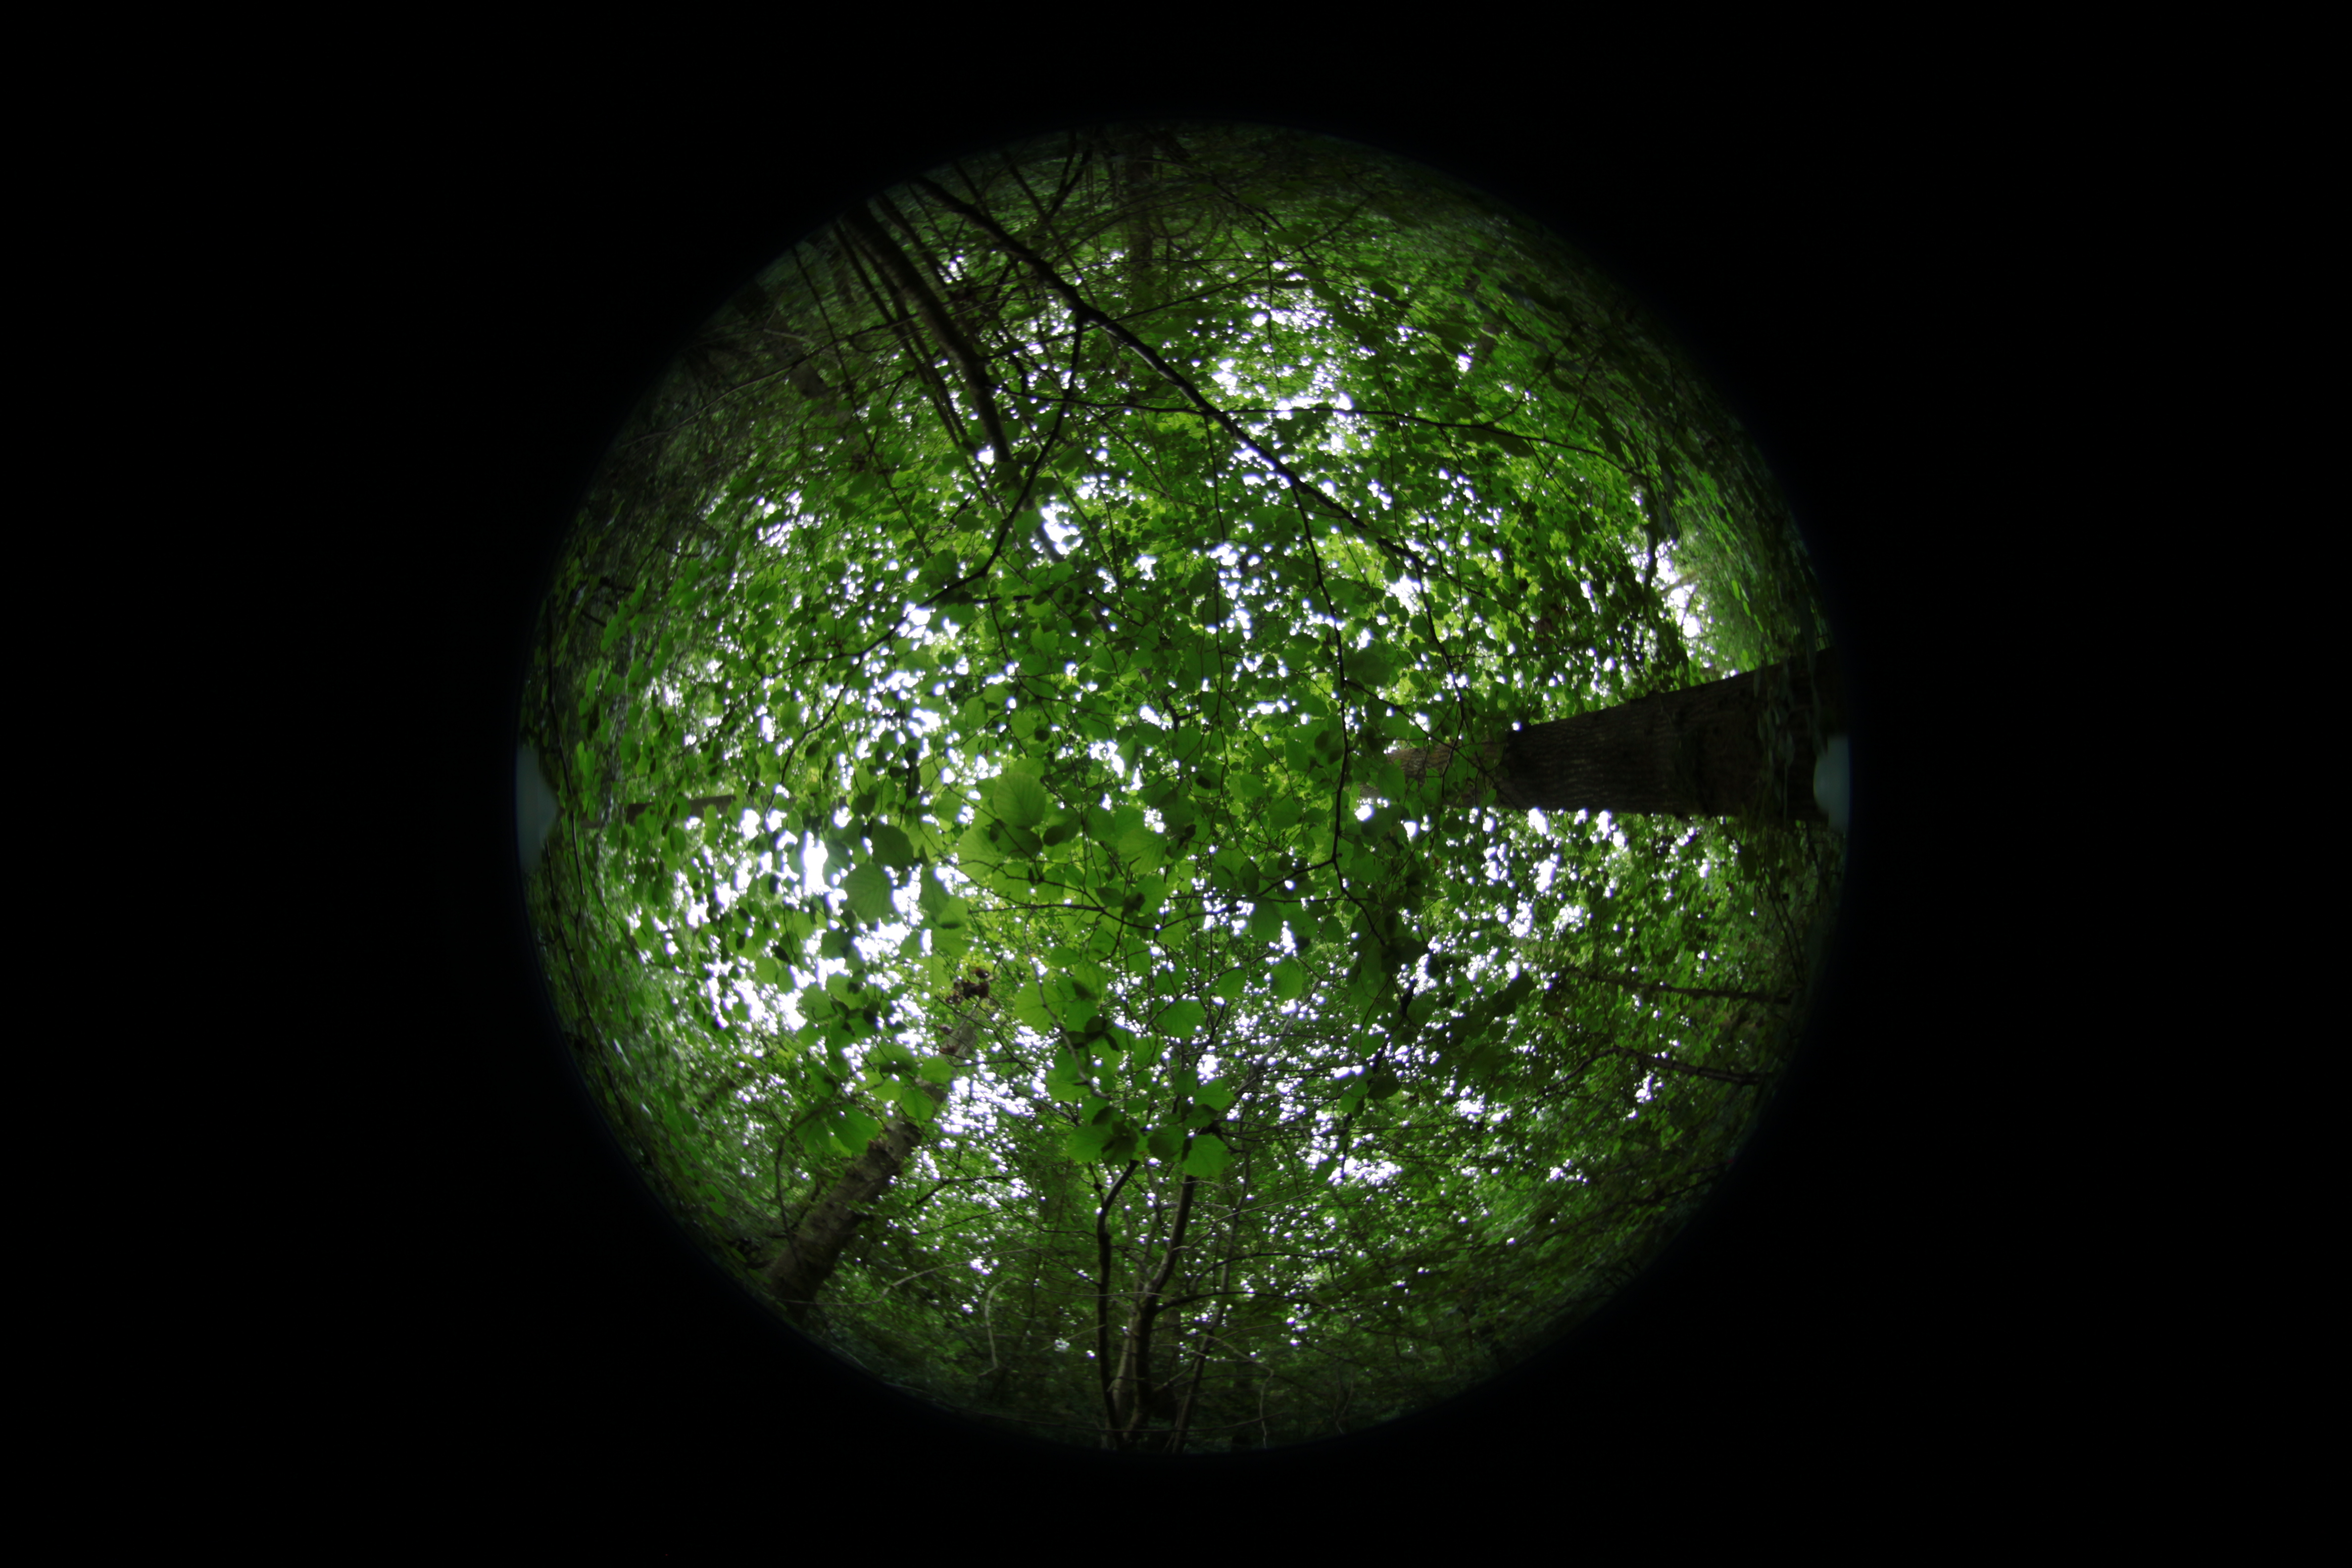
\includegraphics[width=.9\linewidth]{chapter/chapter4/043exp2.jpg}
  \caption{Unthinned forest}
  \label{chap4:fig:sub1}
\end{subfigure}%
\begin{subfigure}{.5\textwidth}
  \centering
  \includegraphics[width=.9\linewidth]{chapter/chapter4/252exp1.jpg}
  \caption{Thinned forest}
  \label{chap4:fig:sub2}
\end{subfigure}
\caption{Hemispherical photographs from the Alice Holt flux site showing the difference between the thinned and unthinned sides of the forest.}
\label{chap4:fig:hemiphotos}
\end{figure}

\subsubsection{Litter traps}

Finally, litter traps were used to find estimates of LAI and leaf mass per area. We placed litter traps under the canopy to catch leaf litter into a bag attached to the bottom of the trap. The bags were changed every week during the litter fall period and the litter sorted into species. Every week the litter was dried in an oven at $70^{\text{o}}\text{C}$ and weighed. This gave us the dry-weight of the leaf litter for the 2015 season. Towards the end of the season we scanned a 100 leaves for each species to find an average leaf area, we then dried and weighed the leaves. We could then find the leaf mass per area for each species and use this to infer the total LAI for each trap (once the whole seasons litter has been collected). This was then normalised for the are of the trap. This method of LAI calculation is the most time consuming.  

A total of six litter traps were established at points along the transects (positions shown in Figure~\ref{chap4:fig:lit_traps}) allowing for comparison with the other methods. The 6 litter traps are not enough to describe the LAI for the research site \citep{kimmins1973some}. We use these litter traps as a point of comparison and validation for the ceptometer and hemispherical photograph estimates of LAI made at the same locations and also for estimates to leaf mass per area. From our litter trap observations we find a leaf mass per area of 29~g~C~m\(^{-2}\) free soluble carbohydrates for both sides of the forest.

\begin{figure}[ht]
    \centering
    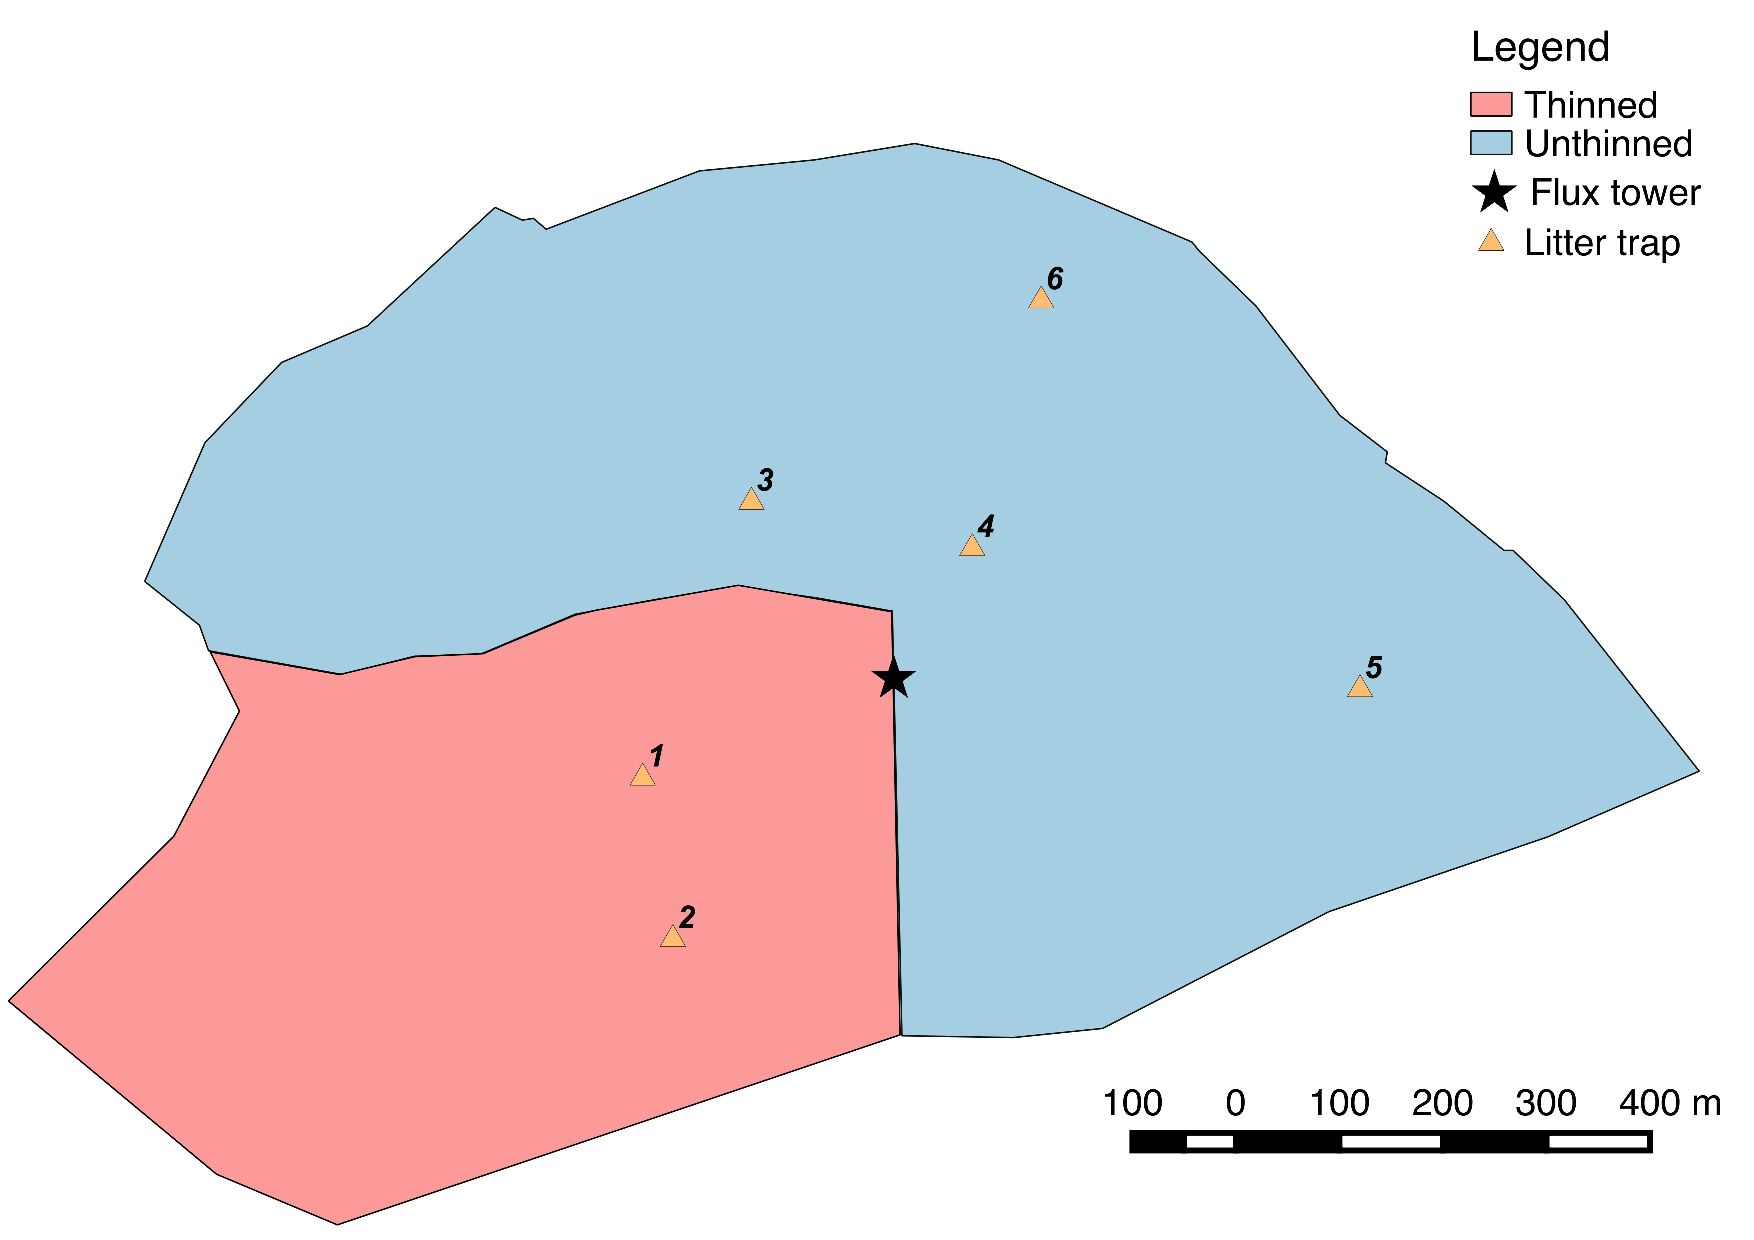
\includegraphics[width=0.8\textwidth]{chapter/chapter4/litter_trap.pdf}
    \caption{Litter trap locations for Alice Holt.} \label{chap4:fig:lit_traps}
\end{figure}


\subsubsection{Comparison of methods} \label{chap4:sec:lai_comp}

In Figure~\ref{chap4:fig:lai_comp07} and \ref{chap4:fig:lai_comp14} we show a comparison of the different methods of estimating LAI for the unthinned and thinned forest respectively. We can see that in all cases LAI derived from the litter traps is always greater than LAI estimated from optical methods, this is expected from previous comparisons \citep{breda2003ground}.
 
Although the ceptometer is the fastest method for measuring LAI it is also the most variable, being extremely sensitive to the solar zenith angle and clear sky conditions. If the sun is low in the sky the radiation will pass through much more photosynthetically active material than if the sun is directly above head, causing spikes in the LAI value. We can see that the LAI estimates from the hemispherical photographs are much less variable than the ceptometer. As discussed in section~\ref{chap4:sec:hemi_photos} the hemispherical estimate is actually of plant area index, as we have not removed trunks and branches from the gap fraction calculation. However, this does not appear to have a great impact on results as hemispherical photograph derived LAI is still the lowest estimate of all three. 

\begin{figure}[ht]
    \centering
    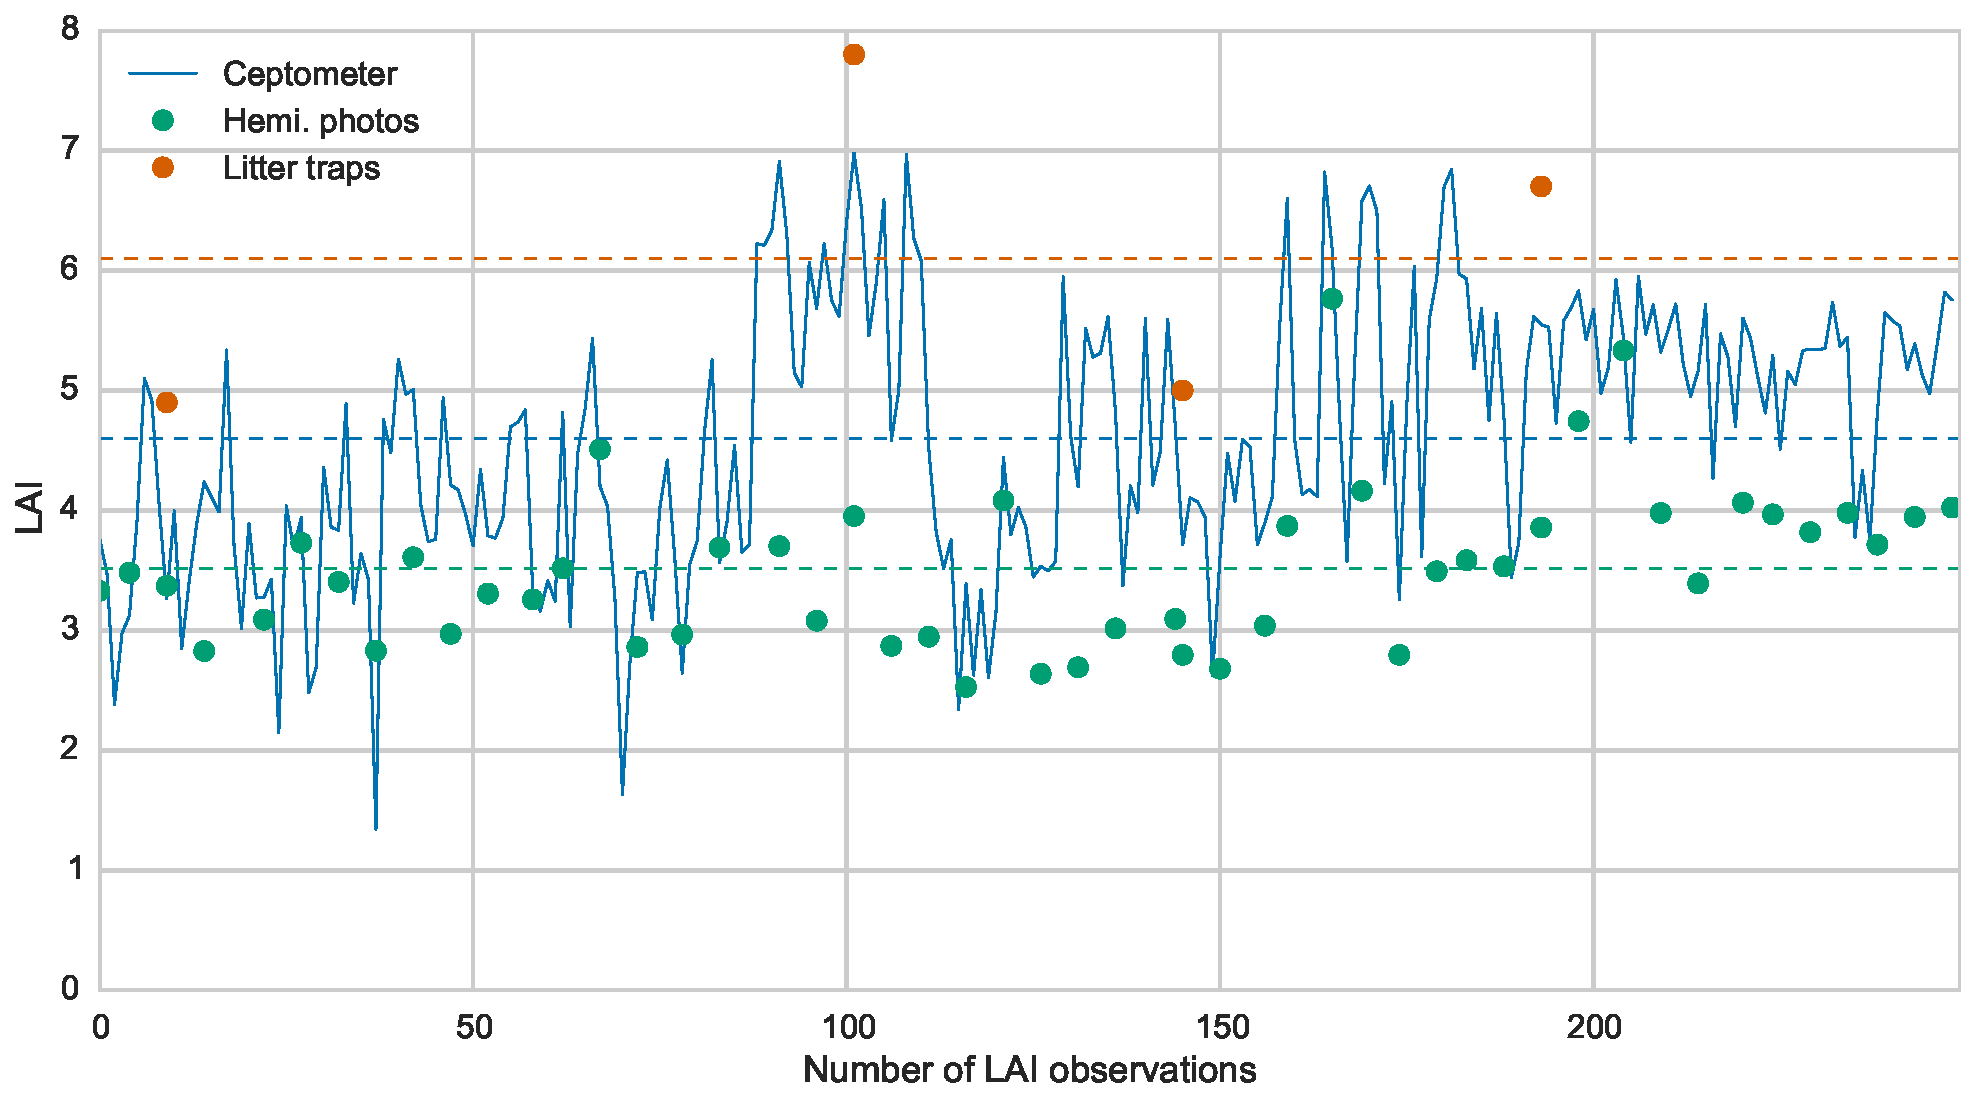
\includegraphics[width=0.8\textwidth]{chapter/chapter4/thinned07.pdf}
    \caption{LAI comparison for unthinned forest. Dots and solid line represent observations made at different points along transects, dotted lines represent the mean of the observations.} \label{chap4:fig:lai_comp07}
\end{figure}

\begin{figure}[ht]
    \centering
    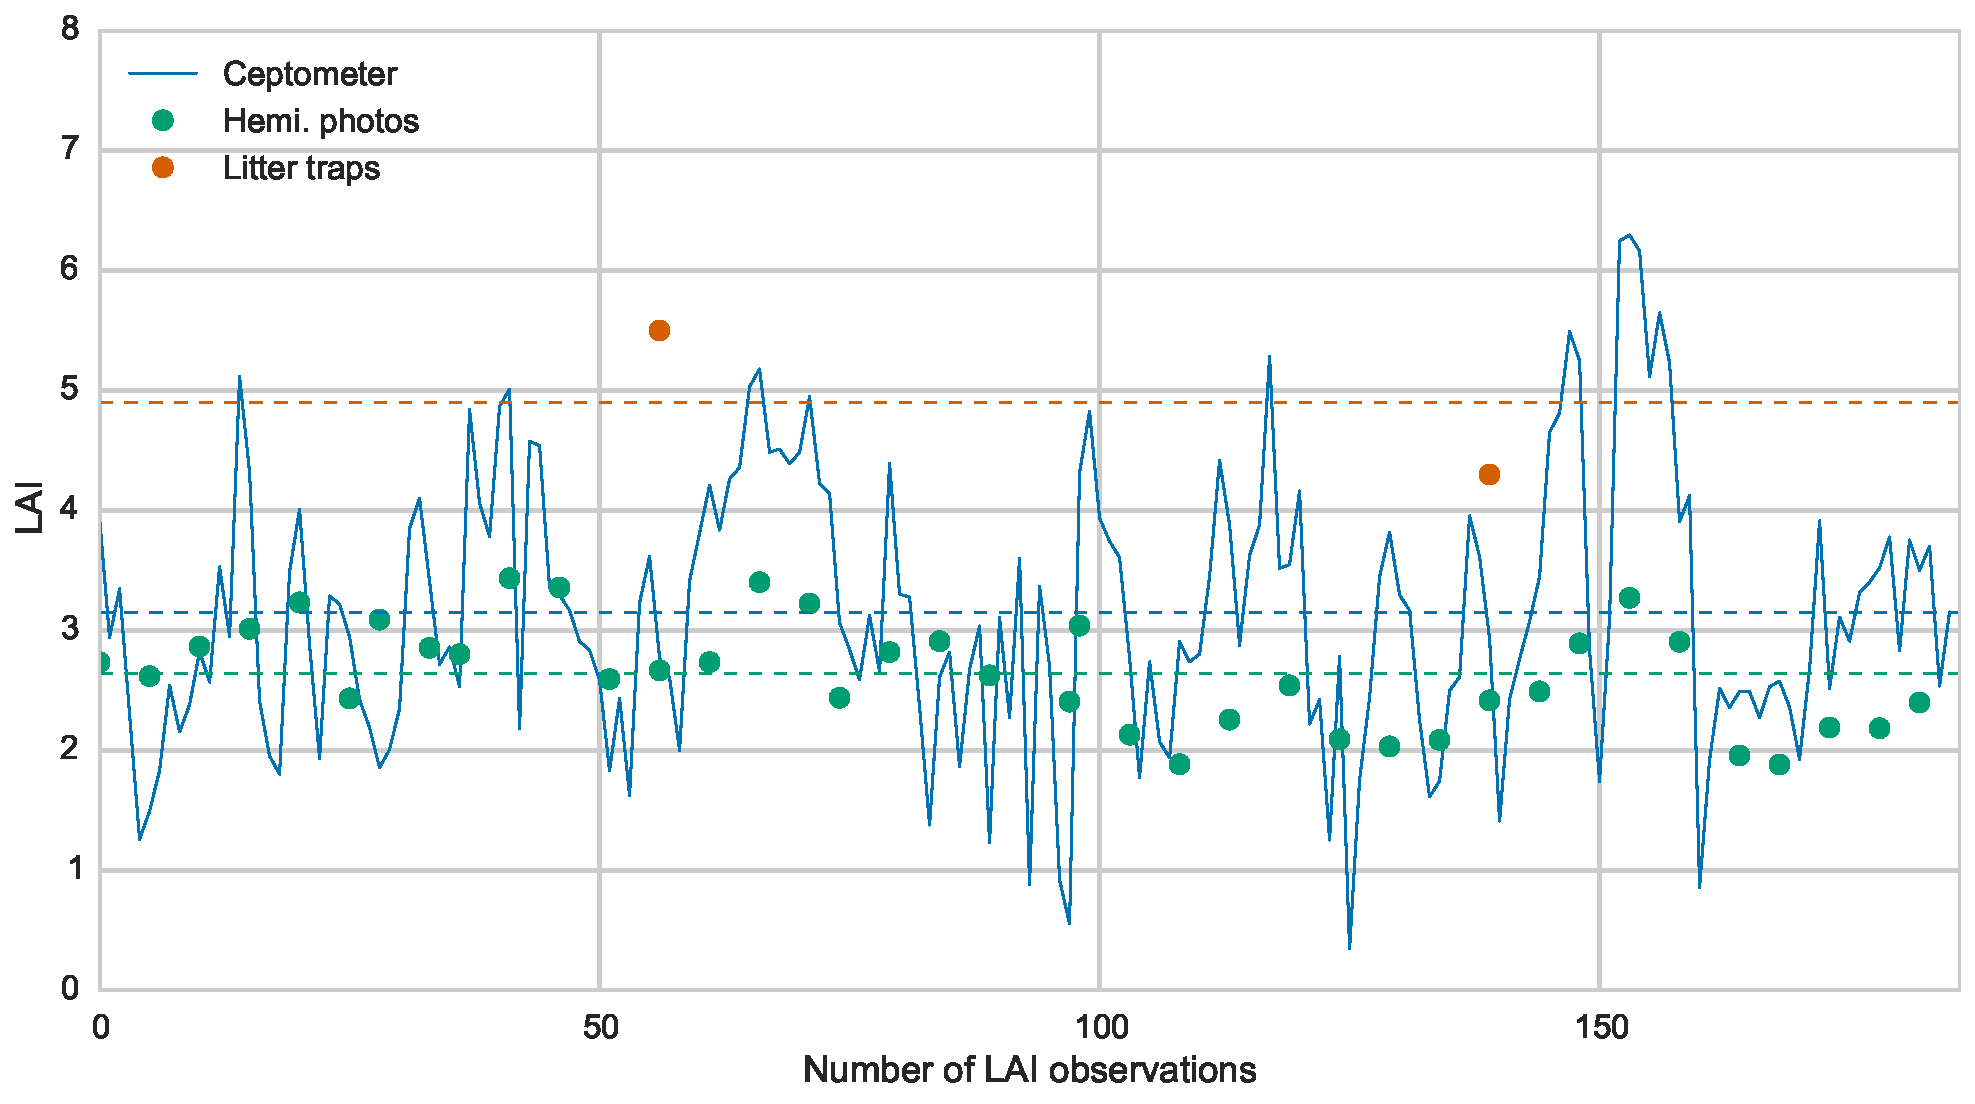
\includegraphics[width=0.8\textwidth]{chapter/chapter4/thinned14.pdf}
    \caption{LAI comparison for thinned forest. Dots and solid line represent observations made at different points along transects, dotted lines represent the mean of the observations.} \label{chap4:fig:lai_comp14}
\end{figure}

\subsection{Point-centred quarter observations} \label{chap4:sec:pcq}

We used the method of Point-Centred Quarters (PCQ) \citep{dahdouh2006empirical} to determine an estimate of the woody biomass for both unthinned and thinned forest in the Straits Inclosure. The PCQ method is conducted at each sampling point as follows:
\begin{itemize}
\item Using a compass, map 4 regions from the central sampling point
\item Measure the distance from the central sampling point to the nearest tree in each quarter
\item Measure the Diameter at Breast Height (DBH) for each tree (shown in Figure~\ref{chap4:fig:dbh_me}) and record the species 
\end{itemize}
There were 114 points sampled along the three transects, from these measurements we derived estimates to tree density and mean DBH for both thinned and unthinned sides of the forest. We then used allometric relationships between DBH and total above ground biomass and coarse root biomass, found in work carried out by Forest Research and in \citet{mckay2003woodfuel}. These relationships were:
\begin{equation}
\text{above ground dry-mass} = 0.0678\times \overline{\text{DBH}}^{2.619}
\end{equation}
and
\begin{equation}
\text{below ground coarse root dry-mass} = 0.149\times \overline{\text{DBH}}^{2.12}.
\end{equation}

This gave us an estimate to the dry-mass in kilograms for the average tree in our sampling area. Assuming that half of all dry-mass is carbon we can find an estimate of total woody and coarse root carbon in g~C~m\(^{-2}\) using the equation,
\begin{multline}
\text{total woody and coarse root carbon} =  \\1000\times0.5\times(\text{above ground dry-mass} + \text{below ground coarse root dry-mass})\times \text{tree density}.
\end{multline}

Forest Research have carried out their own mensuration studies at the site. These have been conducted at the mensuration points shown in Figure~\ref{chap4:fig:transects}. As these plots are included in our transects this means that our measurements should be comparable with those from Forest Research.  

\begin{figure}[ht]
    \centering
    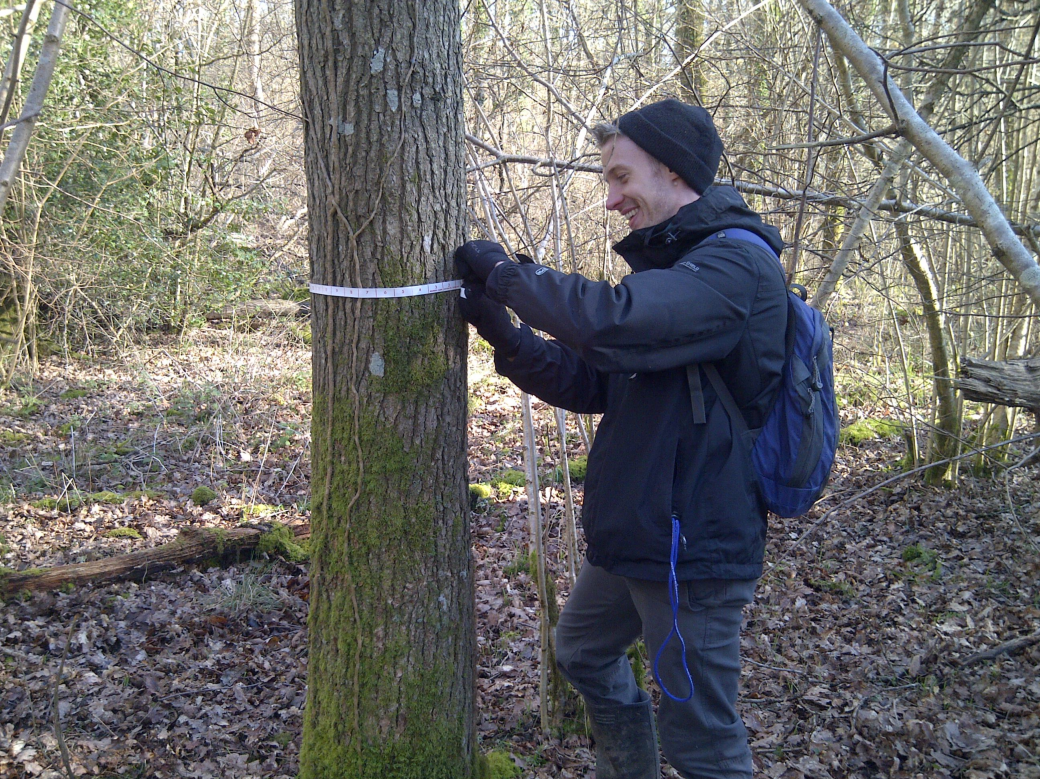
\includegraphics[width=0.8\textwidth]{chapter/chapter4/dbh_me.pdf}
    \caption{Taking diameter at breast height measurements at Alice Holt.} \label{chap4:fig:dbh_me}
\end{figure}

\subsection{Flux tower observations and data processing}

Forest Research provided half-hourly raw flux tower data for the Straits Inclosure from January 1999 to December 2015. These consist of the NEE fluxes and meteorological driving data of temperature, irradiance and atmospheric CO\(_{2}\) concentration for use in the DALEC model. The view from the top of the flux tower in the Straits Inclosure can be seen in Figure~\ref{chap4:fig:flux_me}. Forest Research provided this data in the form of multiple excel spreadsheets corresponding to the flux tower measurement record for each year. To prepare this data for use with data assimilation we first had to convert these 16 excel files to one Python readable data file (here we chose NetCDF), this was then further processed. To process the NEE data we first performed \(u^*\) filtering, where any half-hourly flux observation corresponding to a friction velocity of \(0.2~\text{m s}^{-1}\) or less were removed from the data set. This value represents the point at which Forest Research found flux measurements become unreliable \citep{wilkinson2012inter}. We then subjected the observations of NEE to quality control procedures similar to those described by \citet{papale2006towards}. For each year of the NEE dataset we define two sub-datasets of the half-hourly observations, one containing all positive values and the other all negative values. The standard deviation of both sub-datasets was then calculated. Any values that were \(\pm 3\) standard deviations away from the yearly sub-dataset mean were removed. This was also repeated on a month by month basis. Gap-filling procedures were not applied to the half-hourly NEE dataset so that only true observations were considered for assimilation. To match the time-step of the DALEC model we computed daily NEE observations by taking the mean over the 48 measurements made each day, selecting only days where there was no missing data.   
 

\begin{figure}[ht]
    \centering
    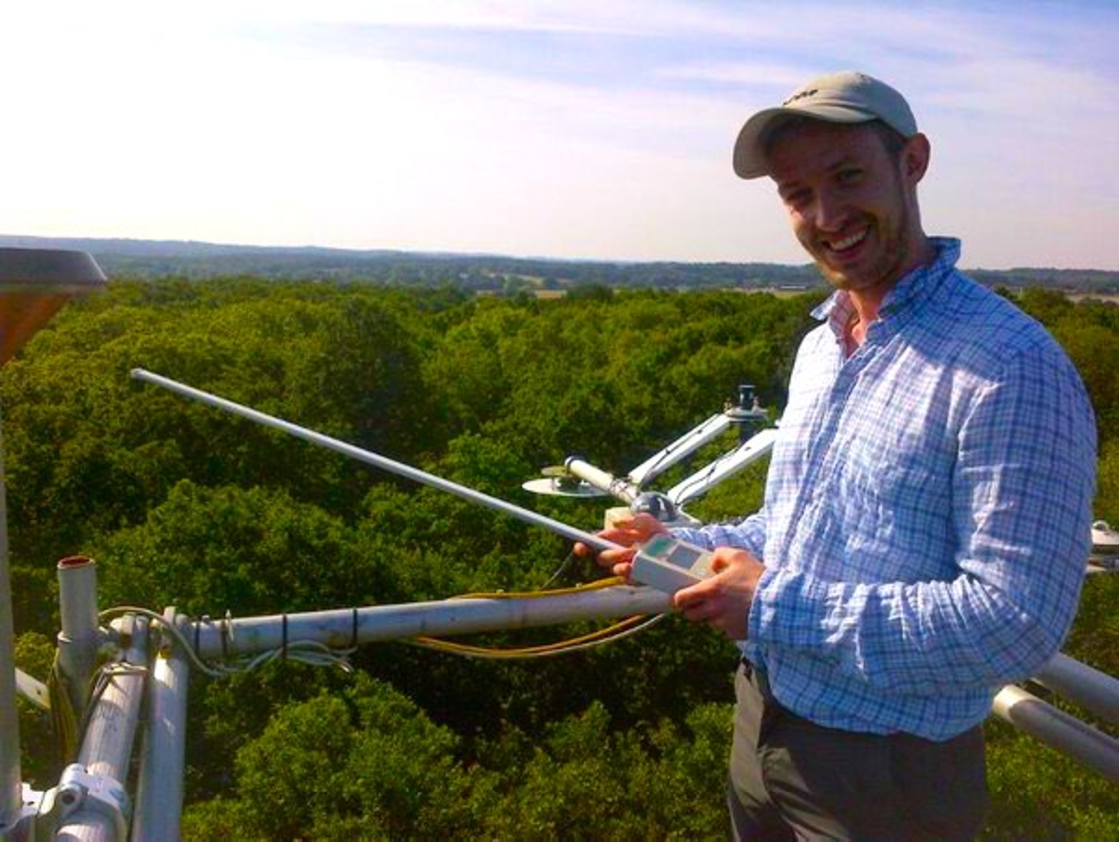
\includegraphics[width=0.8\textwidth]{chapter/chapter4/top_of_flux.pdf}
    \caption{At the top of the Alice Holt flux tower.} \label{chap4:fig:flux_me}
\end{figure}

